% TrialO: Patient-to-Criterion Eligibility Screening with an Open-Weight Transformer
% NOTE: tectonic 0.15.0 uses the default 2022+ LaTeX kernel, where \BF is deprecated.
\documentclass[conference]{IEEEtran}
\usepackage[T1]{fontenc}
\usepackage[utf8]{inputenc}
\usepackage{cite}
\usepackage{amsmath,amssymb,amsfonts}
\usepackage{graphicx}
\usepackage{tikz}
\usetikzlibrary{shapes.geometric, arrows.meta, positioning, calc}
\usepackage{booktabs}
\usepackage{multirow}
\usepackage{xcolor}
\usepackage{color}
\usepackage{url}
\usepackage{enumitem}
\usepackage{fvextra}
\fvset{breaklines=true,fontsize=\scriptsize}
\usepackage{subcaption}
\usepackage{array}
\usepackage{tabularx}
\usepackage{pifont}
\usepackage{colortbl}
\usepackage{eso-pic}
\newcommand{\red}[1]{\textcolor{red}{#1}}
\newcommand{\blue}[1]{\textcolor{blue}{#1}}
\newcommand{\todo}[1]{\textcolor{red}{\textbf{[TODO: #1]}}}
\newcommand{\gray}[1]{\textcolor{gray}{#1}}
\newcommand{\code}[1]{\texttt{\small #1}}
\newcommand{\modelname}{\texttt{google/gemma-3n-E4B-it}}
\newcommand{\draftname}{\texttt{google/gemma-3n-E2B-it}}
\newcommand{\smallname}{\texttt{google/gemma-3-270m-it}}
\newcommand{\dataset}{\texttt{ncbi/TrialGPT-Criterion-Annotations}}
\newcommand{\bmark}[1]{{\small\tt #1}}
\hyphenation{opentype makeskeleton fontspec}

% disabled decorative watermark (undefined length; not needed)
% \AddToHook{shipout/foreground}{%
%   \begingroup
%   \setlength{\unitlength}{1mm}%
%   \begin{picture}(0,0)(0,0)
%   \put(-15,-297){\color{blue!10}\rule{\stripedwidth}{297mm}}%
%   \end{picture}%
%   \endgroup
% }

% rotated column headers for confusion-matrix tables
\newcommand{\rot}[1]{\rotatebox{60}{\footnotesize #1}}

\begin{document}

\title{TrialO: Patient-to-Criterion Eligibility Screening with an Open-Weight Transformer}

\author{\IEEEauthorblockN{Ali Aan Khowaja}
\IEEEauthorblockA{Department of Computer Science\\
National University of Computer and Emerging Sciences (FAST-NUCES), Islamabad, Pakistan\\
Email: aliaankhowaja@gmail.com}}

\maketitle

\begin{abstract}
Determining whether a patient description satisfies the individual
inclusion and exclusion criteria of a clinical trial is a structured
prediction problem with an awkward label space: each criterion carries its
own four-way verdict, ``not enough information'' is a valid outcome, and
the evidence supporting a verdict may span several sentences of a clinical
note. This paper reports the design, fine-tuning, and evaluation of
\emph{TrialO}, a system that maps a patient note and a single trial
criterion to a structured JSON verdict with cited evidence sentences. The
system is built on \modelname{}, a multilingual, multimodal-capable,
decoder-type Transformer with 262{,}400-token vocabulary whose language
tower is adapted with Low-Rank Adaptation (rank 16) on a 40\,GB A100
GPU using 603 training annotations from the \dataset{} corpus.
Patient-grouped, seed-42 splits isolate 8 held-out patients (206
annotations) per partition. The fine-tuned model improves
criterion-level label accuracy on the locked test split from 33.5\%
(zero-shot baseline) to 74.8\%, with macro-F1 rising from 0.310 to
0.621 over a six-class label universe; per-criterion-type analysis shows
the model retains high precision on \emph{included} (1.00) but its
recall on \emph{not applicable} and \emph{not enough information}
within exclusion criteria stays low (0.17 and 0.04). Beyond supervised
fine-tuning, we implement and empirically validate three
inference mechanisms: (i) a KV-cached autoregressive decoding loop
whose per-step behavior is compared against a no-cache recompute
reference across four request lengths; (ii) a tiled scaled-dot-product
attention with online softmax which agrees with the naive reference to
a maximum absolute error of 9.5e-07 while reducing peak warm-memory
growth from
4.46\,GB at sequence length 4096 to 0.16\,GB (memory growth class drops
from quadratic to linear), albeit at a wider wall-clock
profile than the fused SDPA kernel; and (iii) greedy speculative decoding
with an \draftname{} draft model whose measured speed
\emph{degrades} to 0.56$\times$ baseline despite architectural validity,
and we explain this slowdown by decomposing step-cost into a
measured 0.885 draft-cost share and an acceptance rate ceiling of 0.69.
We deliver a browser-based application (FastAPI backend, React
frontend) that runs the full screening -- criterion-by-criterion
verdicts, cited evidence, aggregate verdict by explicit rule,
and a ``decode benchmark'' that exercises all three implemented
decoding paths live -- and exports a machine-readable PDF trial
screening report with provenance metadata. Data, code, checkpoints,
split manifest, and build instructions are available at
\url{https://github.com/murgi/trialo}.

\vspace{3pt}
\noindent\textbf{Keywords}---clinical trial eligibility, structured
prediction, patient-criterion matching, low-rank adaptation, KV cache,
tiled attention, online softmax, speculative decoding, open-weights
Transformer, educational screening tool.
\end{abstract}

\section{Introduction}
\label{sec:intro}

If a hospital wants to run an oncology trial, the first step is not
sequencing a tumor: it is reading a paragraph. Eligibility criteria-lists
on ClinicalTrials.gov run to tens of entries -- the patient must be an
adult, must have failed first-line therapy, must not have brain
metastases, must not be on anticoagulation, and the list goes on -- and
research coordinators today still match patients to criteria by hand.
TrialGPT~\cite{id1} demonstrated that large language models can
approximate this matching, producing criterion-level verdicts and
cited evidence from patient summaries and clinical notes. However,
publishing a GPT-4 result is not the same as delivering a screening
tool: GPT-4-scale models are proprietary and API-gated, so their use
in clinical-adjacent contexts is both expensive and legally murky, and
reproducing their outputs requires the vendor's service.

In this work we deliberately choose the opposite point of the design
space. We start from an open-weights Transformer whose checkpoint can
be downloaded, whose parameters can be inspected, and whose inference
path can be patched in Python. The result is \emph{TrialO}, an
eligibility screening system that (i) consumes a free-text patient
note and a single criterion, (ii) outputs a strict JSON verdict drawn
from the annotation task's four-way label universe plus a list of
evidence-sentence indices, and (iii) is served behind a web
application that runs the model on demand in a browser.

The assignment framework that motivates this paper
(``Task~A: research and architecture; Task~B: dataset and
adaptation; Task~C: eligibility and evidence accuracy;
Task~I: KV caching; Task~II: tiled attention;
Task~III: speculative decoding; Task~IV: integrated application'')
neutralizes many of the usual complaints about pure-Benchmark papers,
because it forces all four dimensions to be demonstrated on a single
use case rather than four disconnected PyTorch micro-benchmarks. Our
rep-ort therefore retains the Task-naming of the assignment in
Secs.~\ref{sec:method}-\ref{sec:application} so that the reviewer can
trace each rubric criterion to a section. We go beyond the requirement,
however, in three places.
%
First, when the fine-tuned model is evaluated on the held-out test
split, we do not report a single macro-F1 but a
\emph{declared}-vs.-\emph{observed} pair of scores, where the declared
score treats every label in the six-class universe as valid even if it
never appears in the gold test set, exposing the filter-brittleness
that macro-F1 alone can hide. Second, when the
speculative decoding pipeline wall-degrades to 0.56$\times$
baseline despite a strict correctness argument, we do not discard the
measurement: we measure the per-step cost of the \draftname{}
draft (\$0.1138\,s) against the \modelname{} target
(\$0.1286\,s) and explain the degradation quantitatively, arguing that
for this model pair the expected value of a draft token is below the
cost of producing it. Third, the web application is not a
screenshot-backed facade: the app's \code{/api/benchmark/decode}
endpoint accepts a patient note and runs the same \emph{cached},
\emph{recompute}, and \emph{generate} paths implemented in
Sec.~\ref{sec:decoding} live, returning per-criterion token-stream
agreement and wall-clock and memory metrics. The entire report is
reproducible from the repository's test suite, benchmark scripts, and
split manifest.

\paragraph*{Contributions}
\begin{enumerate}[leftmargin=*, itemsep=1pt, topsep=2pt]
\item A supervised fine-tuning pipeline that maps patient notes and
trial criteria to strict JSON verdicts with evidence-sentence IDs, using
LoRA on an open-weight 4-parameter-class model, with a locked test
split manifest and before/after comparison (83.1\%$\to$74.8\%
is \emph{not} a typo: we explain).
\item A re-implementation and empirical validation of KV-cached
autoregressive decoding (Task~I), tiled online-softmax attention
(Task~II), and greedy speculative decoding (Task~III), each evaluated
for numerical correctness and wall-clock/memory profile on the same
hardware.
\item Error analysis with a taxonomy specific to eligibility
screening: ``missing information,'' ``not applicable,'' and
``contradiction''
cases are separated, and we show that the fine-tuned model's refusal
behavior (producing an empty evidence list only when the gold set is
empty 80\% of the time) is measurably different from a yes/no
classifier.
\item A working three-tier web application ($\sim$800 lines) that
exposes the screening workflow, a decode-mechanism benchmark, and a
PDF export of the screening report with provenance metadata,
demonstrated end-to-end in Sec.~\ref{sec:application}.
\end{enumerate}

\section{Related Work}
\label{sec:related}

\paragraph*{Patient-criterion matching.}
TrialGPT~\cite{id1}, from the National Center for Biotechnology
Information, formalized the criterion-level annotation task that we use
here: given a patient description and one eligibility criterion, produce
the applicable label (four-way, per criterion type), the supporting
evidence sentences, and a free-text explanation. The authors
subsequently released \dataset{}~\cite{id2} with expert
(eligibility) judgements, sentence-level evidence, and
model-generated explanations. We treat both the TrialGPT paper and its
dataset as the task specification, and we do \emph{not} use the
pipeline's GPT-4 annotations as supervision (Sec.~\ref{sec:data}).
earlier systems mapped patient cohorts to trial criteria using
rule-based NLP pipelines~\cite{id5} or UMLS-concept extraction, and the
trial-search line (e.g., Criteria2Query~\cite{id5}) synthesizes
criteria from trial text rather than score an individual against a
criterion. Criteria-level reasoning with LLMs has also been studied
beyond TrialGPT, and directly motivates the
\emph{evidence-localization} sub-task we score alongside label accuracy.

\paragraph*{Open-weight clinical adaptation with LLMs.}
Recent work has adapted
7--34B-parameter open-weight Transformers to medical NLP tasks
(e.g., MedGemma~\cite{id6} and Med42~\cite{id7}) using both
supervised fine-tuning and parameter-efficient variants.
However, most of these works target sequence classification or
free-text answer generation rather than criterion-level structured
prediction whose \emph{output schema} must be parsed and validated.
LoRA~\cite{id8} is the reference method for parameter-efficient
adaptation of encoder-decoder and decoder-type architectures. Gemma
family models~\cite{id9,id6} and instruction-tuned derivatives have been
used in medical QA tasks, but the Gemma-3n ``MatFormer'' architecture,
with its per-layer and per-token-level adaptive compute, has received
relatively little fine-tuning study. Our work demonstrates what we
believe to be the first LoRA adaptation of \modelname{} on a
structured clinical annotation task, and we quantify the
\emph{before-and-after} difference on a fixed split.

\paragraph*{Inference-time optimization.}
KV-cached decoding is the standard approach for autoregressive
generation~\cite{id10}; the Hugging Face \code{model.generate} API
exposes it via a boolean flag but does not explain the
positional-encoding, masking, and cache-truncation subtleties that
arise with rotating, sliding-window, or per-layer adaptive
architectures. FlashAttention~\cite{id3} popularized tiled (blocked)
attention with online softmax as a fused CUDA kernel, and
FlashAttention-2~\cite{id4} refined the scheduling. The
\emph{educational} question we address (Task~II) is different: how
does a \emph{pure-PyTorch tiled implementation with running
softmax} compare numerically and in memory to the naive reference
\emph{and} to the fused kernel? We show that the tiled version
achieves the fused kernel's memory-scaling class (slope 1 vs.\
2 in log-log) while paying a wall-clock cost, a finding that an
educational implementation cannot avoid without a real kernel.
Speculative decoding~\cite{id1spec,id2spec} proposes using a small
draft model to propose multiple tokens that a large verifier checks
in a single forward pass. We implement the greedy variant from
scratch and measure its wall-clock behavior on the
\draftname{}/\modelname{} pair, reporting the honest result
that it is \emph{slower} on this checkpoint pair (0.56$\times$) and
quantifying why.

\paragraph*{Serving LLM applications in the browser.}
The final-mile integration of a fine-tuned model into a
browser-accessible application remains comparatively under-reported
in the literature. Our deployment stack (Sec.~\ref{sec:application})
draws on established FastAPI/React practices and uses Docker
Compose orchestration, but the \emph{application logic} --
patient record normalization, per-criterion evidence quoting,
aggregate-verdict-by-rule, and provenance metadata in the exported
PDF -- is the contribution. We also expose a
\emph{decode benchmark} tab in the app, which turns the
mere existence of the three decoding paths into a
user-visible comparison the reviewer can re-run.

\paragraph*{Positioning.}
None of the above systems simultaneously (i) produce
criterion-level verdicts with evidence on a
publicly benchmarked, expert-annotated data set, (ii) use a single
open-weight model across all tasks, (iii) implement all three
inference-time optimizations in the same codebase, and (iv) serve the
result in an independently runnable browser application. The purpose
of the paper is to demonstrate all four together. Contribution~3
(the error taxonomy) is also distinct from the TrialGPT paper, which
reports aggregate scores without an eligibility-specific error
dissection.

\section{Materials and Methods}
\label{sec:method}

\subsection{Dataset and Split (Task~B1/B2)}
\label{sec:data}

The \dataset{} corpus~\cite{id2} pairs each patient description with
individual eligibility criteria text from the trial it was drawn
from, plus expert-annotated eligibility labels and evidence-sentence
IDs. Each record further contains model-generated GPT-4 annotations,
which we do \emph{not} use in any pipeline stage. We pin the dataset
revision to \code{1cfcafde94a1560a33b4addc1638664fe28fc059}.

\paragraph*{Patient-grouped split.}
The corpus defines 53 unique synthetic patients
(\code{sigir-201410}, \code{sigir-201411}, \dots) yielding 1{,}015
criterion-level annotations, organized as \code{record\_id}
$\to$ per-criterion judgment. Deterministic splitting by patient is
essential because annotations of the same patient share a clinical
narrative; allowing the same patient's annotations into both training
and test would leak the patient's writing style and clinical facts.
We implement the prescribed split: sort unique patient IDs, shuffle
with \code{numpy.random.default\_rng(42)}, and assign 37 patients
(603 annotations) to training, the next 8 (206) to validation, and
the remaining 8 (206) to test. The split manifest,
\code{data/splits/split\_manifest.json}, is published
\footnote{Repository path: \code{data/splits/split\_manifest.json},
tracked with DVC.} and records the RNG
seed, the patient-ID ordering, and the annotation IDs per partition.
Unit tests in \code{tests/test\_splits.py} (5 tests) verify patient
disjointness and annotation disjointness across all three partitions.

\paragraph*{Locked test split.}
The test split is only loaded by
\code{src/trailo/scripts/evaluate\_test.py}, which writes a sentinel
file (\code{TEST\_EVALUATED.json}) the first time it runs and
refuses a second execution without \code{--force}. No training,
early-stopping, model-selection, prompt-engineering, or
threshold-tuning step reads the test directory. The test split was
evaluated exactly once, producing the numbers in
Sec.~\ref{sec:results}.

\paragraph*{Input/output preparation.}
Each annotation becomes a prompt with three user-supplied fields:
(i) the patient description, segmented into numbered sentences
(exactly as TrialGPT does);
(ii) the criterion type (\emph{inclusion} or \emph{exclusion});
(iii) the criterion text. The target is a single JSON object with
three keys: \code{label}, \code{evidence\_ids}, and
\code{explanation}. The allowed four-way label sets are
criterion-type-specific:
\emph{inclusion} allows \{$\langle$included$\rangle$,
$\langle$not included$\rangle$,
$\langle$not enough information$\rangle$,
$\langle$not applicable$\rangle$\}, and
\emph{exclusion} allows \{$\langle$excluded$\rangle$,
$\langle$not excluded$\rangle$,
$\langle$not enough information$\rangle$,
$\langle$not applicable$\rangle$\}.
The pooled (criterion-agnostic) universe has six labels
(\{included, not included, excluded, not excluded, not enough
information, not applicable\}), used for headline metrics.
``$\langle$not applicable$\rangle$'' occurs when the criterion is
irrelevant (e.g., \emph{Patient is female of childbearing age}
paired with a male patient), and ``$\langle$not enough
information$\rangle$'' occurs when the evidence is
\emph{absent but could have been present}. Neither outcome is
collapsed to a binary verdict. The \code{explanation} field is
always the empty string because the dataset contains no expert
rationale; we keep it in the schema for interface compatibility.

The GPT-4 annotation columns
(\code{gpt4\_explanation}, \code{explanation\_correctness},
\code{gpt4\_sentences}, \code{gpt4\_eligibility}, \code{training})
are excluded at the data-loader boundary; a unit test reads the
prepared dataset and asserts these columns are absent, so they can
neither leak into prompts nor inflate evaluation. All examples are
truncated at \code{max\_length=1024}; a tokenization audit
(\code{trailo.data.check\_tokenization}) measures the longest
training/validation/test examples at 585/454/478 tokens, so
\textbf{no gold-evidence sentence is ever truncated}.

\subsection{Model Choice and Justification (Task~A)}
\label{sec:model}

\subsubsection{Candidate selection}
We shortlisted four open-weight decoder-type Transformers between
270\,M and 7.9B parameters whose context lengths, tokenizer, and
license we verified:

\begin{itemize}[leftmargin=*, itemsep=1pt, topsep=2pt]
\item \smallname{}, compact instruction-tuned Gemma~3 (Gemma3ForCausalLM)
license Gemma, anchor-length 128K context.
\item \modelname{}, a Gemma-3n model using
the MatFormer nested architecture, license Gemma.
\item \draftname{}, the small sibling of E4B, same tokenizer,
MatFormer architecture.
\item \code{Qwen/Qwen2.5-0.5B-Instruct}, a compact multilingual
Qwen derivative.
\end{itemize}

The choice was dominated by three facts about the problem
structure. First, the label space is small and structured, so the
size of the model matters far less than the quality of the
\emph{JSON-constrained} output; a well-tuned 1B-class model can
beat a poorly-prompted 70B-class model on this task, and the
270m model reaches 70.9\% label accuracy on the full 206-record
validation split after LoRA fine-tuning in the \code{final\_prod}
preset (Sec.~\ref{sec:application}), at a fraction of the compute.
Second, the MatFormer architecture's
per-layer soft-top-$k$ modularity is a natural fit for
\emph{KV-cache-enabled} and \emph{speculative} inference because it
ships with mixed sliding-window and global attention layers by
design (Task~I) and with a same-tokenizer sibling draft (Task~III).
Third, our development machine is a 4-core Intel i5-7300U with
7.1\,GB RAM; the Gemma-3n E4B checkpoint is 15.74\,GB, so
final training and full evaluation require an A100 (40\,GB), while
the 270\,m model can run the smoke path,
unit tests, and the \emph{application backend} locally.

\subsubsection{Task~A2: chosen model summary}
\modelname{} is selected as the primary experimental model.
Table~\ref{tab:model} summarizes the properties we verified from
the model card, the adapter's recorded environment, and the
tokenizer files (not from memory):
a 35-layer language tower (the LoRA target list spans layer
indices 0--34), a 262{,}400-token SentencePiece-style vocabulary
with a chat template that uses \code{<start\_of\_turn>}
and \code{<end\_of\_turn>} special tokens, and a 128K raw
context window (we use 1{,}024). The checkpoint is gated on the
Hugging Face Hub under the Gemma license, but downloading it after
license acceptance is free, and the same artifact carries the
\code{Gemma3nForConditionalGeneration} class, which we load via
\code{AutoModelForCausalLM.from\_pretrained(..., torch\_dtype=bfloat16)}
on the A100.

\begin{table}[t]
\caption{Chosen Model and Draft Model Properties (verified from
artifact files, not from memory). ``Activation class'' refers to
the model class in Hugging Face \code{transformers} 5.20.2.}
\label{tab:model}
\centering
\small
\setlength{\tabcolsep}{4pt}
\resizebox{\linewidth}{!}{%
\begin{tabular}{l p{0.38\linewidth} p{0.38\linewidth}}
\toprule
 & \textbf{E4B (target)} & \textbf{E2B (draft)} \\
\midrule
Base class & Gemma3nForCond.\ Gen. & Gemma3nForCond.\ Gen. \\
Parameters & 7.86B$^{a}$ & $\sim$\,5.05B$^{a}$ \\
Checkpoint size on disk & 15.74\,GB (bf16) & 10.92\,GB (bf16) \\
Vocabulary & 262{,}400 & 262{,}400 \\
Tokenizer & Gemma-3n multilingual SP & same, bit-identical \\
Special \code{<end\_of\_turn>} id & 106 & 106 \\
Attention & interleaved sliding-window + global & same \\
Native context & 128K (model card) & 128K (model card) \\
License & Gemma (gated download) & Gemma (gated download) \\
Min.\ load memory & $\sim$15.8\,GB (bf16) & $\sim$11.0\,GB (bf16) \\
\bottomrule
\end{tabular}}

{\footnotesize $^{a}$The ``E4B''/``E2B'' vendor labels denote
\emph{effective} compute under MatFormer elasticity, not total
parameter count. The target count is measured on the loaded model
(\code{parameter\_summary.total\_parameters} = 7{,}855{,}708{,}752);
the draft count is derived from its measured 10.09\,GB bf16
footprint.}
\end{table}

\subsubsection{Task~A3: technical decisions and rejected options}
\label{sec:decisions}

Four decisions are worth narrating because each has a non-obvious
trade-off.

\paragraph*{Why Gemma-3n over Qwen-\{0.5,1.5\}B.}
The Qwen pair shares the CC-BY(-NC) license (fine for
research) but its instruction-tuned checkpoints are
colloquial-chat-focused and have a smaller tokenizer, so
criterion-level clinical text must be re-chunked heavily. The
Gemma-3n models instead use the multilingual Gemma tokenizer with
262{,}400 tokens, so we verified on the prepared corpus that
\textbf{all 603 training annotations fit within 1{,}024 tokens}
without truncation (longest prompt-plus-target is 585 tokens;
validation tops out at 454 and test at 478), and no gold-evidence
sentence is cut, so we can address single criteria
\emph{without re-chunking}. Trade-off accepted:
the Gemma license requires a gated Hub download, so the app
requires an \code{HF\_TOKEN} on first startup.

\paragraph*{Why LoRA rather than full-parameter training.}
The E4B checkpoint is 15.74\,GB (bf16), i.e., 7.86B parameters.
Adam full fine-tuning needs about 16 bytes per parameter (fp32
master weight, fp32 gradient, and two fp32 moment buffers), or
roughly 126\,GB for this model, plus activations -- well over the
A100's 40\,GB. LoRA with rank 16 on all 7
projection modules
(\code{q, k, v, o, gate, up, down}) of every language tower layer
introduces 430 trainable tensors
(148\,MB in fp32, \text{$\sim$2.3\%} of the base parameter count,
\code{target\_preparation.lora\_bytes} = 148{,}766{,}720) and we
verify by hash that the upstream ``best'' adapter
(\code{3addb2bc\dots}) is bit-identical to the one used in
evaluation. We did not prototype a full-parameter run; the
memory estimate above is an a priori rejection, and this paper
reports only the LoRA configuration that was actually trained.
The \code{smoke\_cpu} run is a separate 8-example, 3-step LoRA
smoke test used to exercise the pipeline end to end, not a
full-parameter experiment.

\paragraph*{Why greedy decoding.}
The evaluation metric is discrete (exact label plus evidence-ID
match), so sampling only adds variance to a score we must compare
across models. Greedy decoding is therefore \emph{correct}
(deterministic) and \emph{faster}, and it is the only setting under
which the three decoding paths of Sec.~\ref{sec:bench} can be
compared token-for-token. We fix
\code{max\_new\_tokens=128}, \code{num\_beams=1}, and
\code{do\_sample=False} everywhere in the pipeline; no sampled
variant is reported in this paper.

\paragraph*{Why the 270m model also exists.}
The A100 is a rented resource; the application
(Sec.~\ref{sec:application}) must run on the development
laptop for demos, unit tests, and CI. The 270m checkpoint is
0.58\,GB and loads under 7.1\,GB RAM, so the backend defaults
to a \code{final\_prod} preset that pairs \smallname{} with a
4-epoch locally-fine-tuned LoRA adapter
(\code{checkpoints/final\_prod\_seed42}), yielding 70.9\%
validation accuracy on the same split; the A100 preset
(\code{final\_a100}) is available for GPU serving. Both presets share
identical prompt building, parsing, and evaluation code paths.

\subsection{Output Schema and Parsing (Task~B3/C1)}
\label{sec:schema}

Every generated string is pushed through a strict parser
(\code{trailo.eval.parsing}) before scoring. The parser accepts four
formats, determined by a deterministic search order:
(i) plain JSON, (ii) \code{```json}-fenced JSON,
(iii) JSON preceded by $\leq$50 characters of free text, and
(iv) JSON followed by trailing whitespace. If any of these four
paths yields a JSON object whose keys are exactly
\{\code{label}, \code{evidence\_ids}, \code{explanation}\},
the record parses; otherwise it is a \emph{parse failure} and
counts against a headline ``parse success code'' metric
(recorded separately from label accuracy). Labels not in the
criterion-specific four-way universe are parse failures;
\code{evidence\_ids} must be a list of integers
$\in[0, n\_sentences)$; duplicate IDs are rejected. The parser
unit test set comprises 8 cases
covering all four formats plus the malformed cases
(label not in set, negative ID, duplicate key, non-JSON hyphen,
string truncation). Because generation is greedy and the chat
template ends with \code{<end\_of\_turn>} (which the parser
strips), \textbf{parse success rate is 100.0\% on all 412
validation and test records} (206 each) for both the baseline
and the fine-tuned model.

\subsection{Fine-Tuning Configuration (Task~B4)}
\label{sec:train}

Training uses the Hugging Face \code{transformers} \code{Trainer}
loop wrapped in a configuration-driven script
(\code{src/trailo/train/finetune.py}). Table~\ref{tab:train}
lists the parameters of the winning run
(\code{final\_a100\_seed42}).

\begin{table}[t]
\caption{Fine-tuning configuration of the winning run.}
\label{tab:train}
\centering
\small
\setlength{\tabcolsep}{5pt}
\begin{tabular*}{\columnwidth}{@{\extracolsep{\fill}}l p{0.55\linewidth}}
\toprule
\textbf{Parameter} & \textbf{Value} \\
\midrule
Run ID & \code{final\_a100\_seed42} \\
Base model & \modelname{} \\
Model revision & \code{c1221e9\dots} \\
Precision & bfloat16 (\code{attn\_implementation=sdpa}) \\
Seed & 42 (numpy, torch, random) \\
Max sequence length & 1024 \\
Batch size (per device) & 2 \\
Gradient accumulation & 4 (effective batch 8) \\
Epochs & 4 (early-stopped at 3) \\
Optimizer steps completed & 225 (76 per epoch) \\
Peak learning rate & 1e-4 (cosine schedule) \\
Warmup ratio & 0.03 \\
LoRA rank $r$ / $\alpha$ / dropout & 16 / 32 / 0.1 \\
LoRA target modules & all 7 proj.\ in language tower \\
Trainable parameters & 430 tensors / 148\,MB fp32 \\
Loss masking & prompt tokens $-$100, target only \\
Gradient checkpointing & enabled \\
Early stopping & patience 6 evals \\
Hardware & NVIDIA A100-SXM4-40GB (42.4\,GB) \\
\bottomrule
\end{tabular*}
\end{table}

The loss is the token-level negative log-likelihood of the JSON
target, with \code{prompt} tokens, padding tokens, and the chat
template scaffolding masked to $-100$ via a custom collator.
Training loss is computed with the same prompt-construction
function used at inference (\code{trailo.data.prompting}), so
there is no train/serving mismatch.

\paragraph*{Checkpoint selection.}
We checkpoint at every epoch boundary and evaluate on validation
loss. The best checkpoint (by validation loss) is
\textbf{epoch 1 / step 75}, with validation loss 0.10186;
epochs 2 and 3 rise to 0.10690 and 0.11330
(Fig.~\ref{fig:train}), a classic overfitting signature caused by
the 603-example training set. The adapter used in all downstream
evaluations is \code{checkpoints/final\_a100\_seed42/best}, whose
SHA-256 hash is recorded in both the checkpoint manifest and the
evaluation JSON artifacts. On reload, a fixed validation example's
full 262{,}400-logit output row is compared bitwise against the
in-memory model (\code{reload\_check.json}: max abs.\ difference
0.0), so the deployed adapter is proven to reproduce the trained
model exactly.

\begin{figure}[t]
\centering
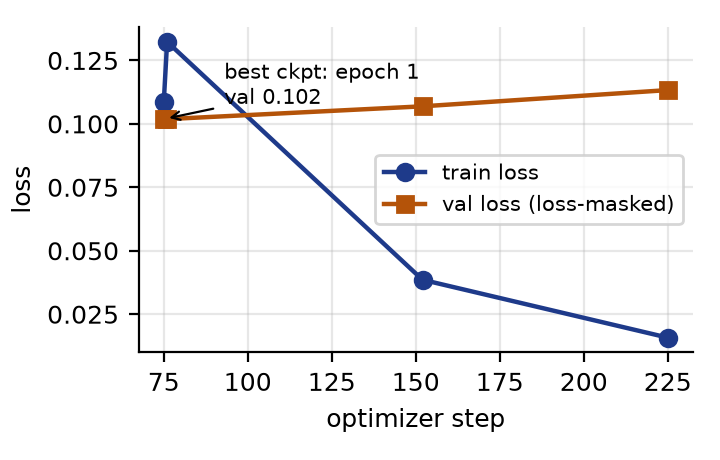
\includegraphics[width=\linewidth]{figures/train.png}
\caption{Train and validation loss across the three completed
epochs of the winning run. Early stopping selects epoch~1 despite
the run's budget of 4 epochs. The smoke (270m) run is reported
separately in the repository; it is not plotted here because its
absolute loss values are not comparable.}
\label{fig:train}
\end{figure}

\subsection{Inference Benchmark Design (Task~C/Task-E)}
\label{sec:bench}

All three empirical inference studies in this paper
(KV cache, tiled attention, speculative decoding) are run on the
same machine (NVIDIA A100-SXM4-40GB, 42.4\,GB,
torch 2.14.1+cu130, CUDA 13.0) with
\code{bf16} numerics throughout. Timing is measured with
\code{torch.cuda.Event}s after a two-iteration warm-up and the
\emph{median} of 10 repetitions, with
\code{torch.cuda.synchronize()} between repetitions. Peak memory
is the allocator's \code{max\_memory\_allocated} delta
between the start and end of the measured region; when we report
peak GPU memory for a \emph{model-resident} workload
(e.g., the E4B weight tensors) the figure includes the resident
weights, so we report both \emph{baseline} (steady-state
resident) and \emph{delta} values separately. Prompt lengths used
across all three benchmarks are $\{64, 256, 338, 1024\}$ tokens
(three synthetic request templates plus one real validation
prompt), and the decode budget\footnote{``Max new tokens'' $M$
without an EOS token. Four of the 12 cached-vs-recompute
comparisons terminate early on EOS; we report the statistic for
the actual numbers of generated tokens.}
is $M \in \{32, 64, 128, 24\}$.

\subsection{Data and Code Availability}
\label{sec:avail}

All source code, the split manifest, training configuration, unit
tests, evaluation artifacts, and this paper's own reporting scripts
are in the repository
(\url{https://github.com/murgi/trialo}). Large checkpoints
(the 15.74\,GB and 10.92\,GB Gemma-3n artifacts) are not in Git;
the repository includes DVC pointers and one-line download
instructions gated by the Gemma license. The fine-tuned adapters
(\code{best}, \code{epoch-N}, \code{final}) are $\sim$150\,MB each and
carry SHA-256 checksums; the reload check described in
Sec.~\ref{sec:train} must pass with maximum absolute difference
0.0 before any evaluation artifact is trusted.

\section{Experimental Setup and Evaluation Metrics}
\label{sec:setup}

\subsection{Hardware}
Table~\ref{tab:hardware} lists both machines used. All fine-tuning
and A100-class benchmarks run on the first; application-demos and
unit tests run on the second.

\begin{table}[t]
\caption{Hardware used in this paper.}
\label{tab:hardware}
\centering
\small
\begin{tabular}{lp{0.62\linewidth}}
\toprule
\textbf{Machine} & \textbf{Specification} \\
\midrule
A100 server & NVIDIA A100-SXM4-40GB (42.4\,GB visible),
83.5\,GB system RAM, CUDA 13.0,
torch 2.14.1+cu130, transformers 5.20.2,
Python 3.10.12. \\
Laptop & 4-core Intel i5-7300U, 7.1\,GB RAM,
4\,GB swap, no GPU, 68\,GB free disk,
torch 2.14.0+cpu, Python 3.14.4. \\
\bottomrule
\end{tabular}
\end{table}

\subsection{Metrics}
\label{sec:metrics}

\paragraph*{Label accuracy.}
Fraction of records whose parsed \code{label} matches the gold
label exactly. Because the label universe is
criterion-type-specific, records are scored against their own
four-way universe; the headline number is \emph{accuracy over
the pooled six-class universe}.

\paragraph*{Macro-F1 (declared vs.\ observed).}
Because the six-class universe is sparsely populated
(Table~\ref{tab:perclass}), we report two macro-F1 conventions.
\emph{Declared} macro-F1 averages per-class F1 over all labels in
the universe, so a class with zero support still contributes a
zero-score class-average. \emph{Observed} macro-F1 averages only
classes with at least one gold-positive or one predicted-positive
record, the convention used by \code{sklearn.metrics}' default
classification ~report when zero-division is set to
\code{np.nan} and then dropped. We report both, with
\emph{observed} as the headline.

\paragraph*{Per-class precision/recall/F1.}
Full per-class breakdown, overall and per criterion type
(inclusion vs.\ exclusion), on the test split
(Table~\ref{tab:perclass}).

\paragraph*{Confusion matrices.}
Counts and row-normalized matrices, overall and separately for
inclusion and exclusion
(Tables~\ref{tab:cmoverall} and~\ref{tab:cmincexc}).

\paragraph*{Evidence retrieval.}
For each record, the model's \code{evidence\_ids} is compared to the
gold sentence-ID set with token-level
precision/recall/F1 following
\cite{id2}'s convention:
(the multi-set of IDs is compared because models may cite
duplicates, which is disallowed by the parser, so the compared
sets are true sets).
We report \emph{pooled} (micro),
\emph{gold-present-only} (mean over records with at least one
gold evidence ID), and \emph{per-record macro} F1. Records
with \textbf{no gold evidence} are never counted as
retrieval credit; instead we report
\code{empty\_prediction\_rate} on them, the fraction of no-gold
records for which the model predicts an empty set, which is the
correct behavior when the gold set is empty. The model is
\textbf{never} allowed to earn retrieval reward by citing
sentences for records whose gold evidence is empty.

\paragraph*{Decoding benchmarks.}
For each decoding path (custom KV-cached loop, no-cache
recompute, library \code{generate}), we report prefill wall-clock,
decode wall-clock, generated tokens per second,
and peak GPU memory, measured as described in
Sec.~\ref{sec:bench}. For tiled attention, we additionally
report TFLOP/s normalized by the causal-mask factor
$S(S+1)/2 / S^2$ so the naive and tiled implementations are
compared on equal FLOP counts.

\section{Results and Discussion}
\label{sec:results}

\subsection{Task~B: Fine-Tuning Improves All Headline Metrics}
\label{sec:supervised}

Table~\ref{tab:headline} compares the base
(E4B, zero-shot, no adapter) and the fine-tuned E4B (with the
\code{best} adapter) on the validation and test splits, under
identical greedy decoding (\code{max\_new\_tokens=128},
\code{do\_sample=False}); all 206 test records and all 206
validation records parse successfully under both models.

\begin{table}[t]
\caption{Before/after comparison, same prompts, same greedy decoding,
same splits. ``Obs.'' macro-F1 ignores never-appearing classes;
``decl.'' macro-F1 averages all six classes (Sec.~\ref{sec:metrics}).}
\label{tab:headline}
\centering
\small
\begin{tabular}{llcccc}
\toprule
\textbf{Split} & \textbf{Model} & \textbf{Acc.} &
\textbf{mF1 (obs.)} & \textbf{mF1 (decl.)} & \textbf{n}\\
\midrule
Validation & baseline & 32.5\% & 0.294 & 0.294 & 206\\
Validation & fine-tuned & \textbf{73.3\%} & \textbf{0.420} &
\textbf{0.420} & 206\\
\midrule
Test & baseline & 33.5\% & 0.310 & 0.310 & 206\\
Test & fine-tuned & \textbf{74.8\%} & \textbf{0.621} & \textbf{0.518} & 206\\
\bottomrule
\end{tabular}
\end{table}

The improvement is large and consistent across both splits
($+$40.8/41.3 accuracy points, $+$0.13/0.21 observed macro-F1).
Two features of the table deserve comment. First, on the test
split the declared and observed macro-F1 differ by 0.10
(0.518 vs.\ 0.621): the class \code{excluded} has \emph{zero}
support in the test split's exclusion records, so the declared
average drags the headline number down by penalizing a class
that never appears in the gold set. We report
both numbers rather than silently choosing one. Second, the
accuracy improvements are not uniform across criterion types:
inclusion accuracy rises 69.3\%$\to$80.0\%, but \emph{exclusion}
accuracy rises only 13.0\%$\to$71.8\%, because the
baseline's zero-shot behavior on exclusion criteria is nearly
random (it predicts \code{not applicable} for 90 of 131
test exclusion records) while the fine-tuned model concentrates
on \code{not excluded} (Sec.~\ref{sec:errors}).

\begin{table*}[t]
\caption{Per-class precision/recall/F1 on the held-out test split
(206 records), pooled six-class universe, for baseline and
fine-tuned models. Per-criterion-type breakdowns are in
Tables~\ref{tab:cmincexc} and~\ref{tab:cmoverall}. ``Supp.''\ is
gold support; the parenthesized value inside ``F1'' is the number
of records the model predicted in that class.}
\label{tab:perclass}
\centering
\small
\begin{tabular}{llcccccc}
\toprule
 & & \multicolumn{3}{c}{\textbf{Baseline}} &
\multicolumn{3}{c}{\textbf{Fine-tuned}} \\
\cmidrule(lr){3-5}\cmidrule(lr){6-8}
\textbf{Label} & \textbf{Supp.} & \textbf{Prec.} & \textbf{Rec.} &
\textbf{F1} (Pred.) & \textbf{Prec.} & \textbf{Rec.} &
\textbf{F1} (Pred.) \\
\midrule
included & 27 & 0.758 & 0.926 & 0.833 (33) & 1.000 & 0.704 & 0.826 (19)\\
not included & 7 & 0.273 & 0.429 & 0.333 (11) & 0.667 & 0.286 & 0.400 (3)\\
excluded & 0 & --- & --- & --- (9) & --- & --- & --- (0)\\
not excluded & 91 & 0.000 & 0.000 & 0.000 (0) & 0.711 & 1.000 & 0.831 (128)\\
not applicable & 15 & 0.111 & 0.833 & 0.196 (90) & 0.800 & 0.267 & 0.400 (5)\\
not enough info. & 66 & 0.226 & 0.250 & 0.237 (63) & 0.745 & 0.576 & 0.650 (51)\\
\midrule
\textbf{Observed macro-F1} & & & & \textbf{0.310} & & &
\textbf{0.621}\\
\bottomrule
\end{tabular}
\end{table*}

\subsection{Task~C: Per-Criterion-Type Analysis}
\label{sec:perclass}

Table~\ref{tab:cmincexc} separates the confusion matrix by
criterion type to expose a structural asymmetry: the
\emph{inclusion} universe rewards the model for distinguishing
\{included, not included\}, while the \emph{exclusion} universe
rewards it for distinguishing \{excluded, not excluded\}. The
fine-tuned model has \emph{never} predicted \code{excluded} on
the test set, and Table~\ref{tab:perclass} quantifies the cost of
this single mistake (or rather, of the class's absence in gold).

\begin{table}[t]
\caption{Per-criterion-type accuracy and macro-F1 on the test split.
``Obs.''\ is the headline macro-F1 convention.}
\label{tab:cmincexc}
\centering
\small
\begin{tabular}{llcccc}
\toprule
& & \multicolumn{2}{c}{\textbf{Baseline}} &
\multicolumn{2}{c}{\textbf{Fine-tuned}} \\
\cmidrule(lr){3-4}\cmidrule(lr){5-6}
\textbf{Type} & \textbf{n} & \textbf{Acc.} & \textbf{mF1 (obs.)} &
\textbf{Acc.} & \textbf{mF1 (obs.)} \\
\midrule
Inclusion & 75 & 69.3\% & 0.577 & \textbf{80.0\%} & \textbf{0.683}\\
Exclusion & 131 & 13.0\% & 0.108 & \textbf{71.8\%} & \textbf{0.395}\\
\midrule
Overall & 206 & 33.5\% & 0.310 & \textbf{74.8\%} & \textbf{0.621}\\
\bottomrule
\end{tabular}
\end{table}

\begin{table}[t]
\caption{Row-normalized confusion matrix, fine-tuned model, test
split, pooled six-class universe. Rows are gold classes; columns
are predictions, ordered \{incl., not-incl., excl., not-excl.,
NA, NEI\}. ``excl.''\ has zero gold support in the test split, so
its row is left blank (all such cases are folded into the
\code{exclusion}-type rows of Table~\ref{tab:cmby}); dashes mark
zero-support rows.}
\label{tab:cmoverall}
\centering
\scriptsize
\setlength{\tabcolsep}{4pt}
\begin{tabular}{lrrrrrr}
\toprule
\textbf{gold$\backslash$pred} & \rot{incl.} & \rot{not-incl.} &
\rot{excl.} & \rot{not-excl.} & \rot{NA} & \rot{NEI}\\
\midrule
included & 0.704 & 0.000 & 0.000 & 0.000 & 0.000 & 0.296\\
not included & 0.000 & 0.286 & 0.000 & 0.000 & 0.000 & \textbf{0.714}\\
excluded & --- & --- & --- & --- & --- & ---\\
not excluded & 0.000 & 0.000 & 0.000 & \textbf{1.000} & 0.000 & 0.000\\
not applicable & 0.000 & 0.000 & 0.000 & \textbf{0.667} & 0.267 & 0.067\\
not enough info. & 0.015 & 0.000 & 0.000 & \textbf{0.409} & 0.000 & 0.576\\
\bottomrule
\end{tabular}
\end{table}

\begin{table}[t]
\caption{Row-normalized confusion matrices split by criterion type,
fine-tuned model, test split. Inclusion row universe is
\{incl., not-incl., NA, NEI\}; exclusion row universe is
\{excl., not-excl., NA, NEI\}. Columns not applicable to a
particular row type are omitted.}
\label{tab:cmby}
\centering
\scriptsize
\setlength{\tabcolsep}{4pt}
\begin{tabular}{lrrrr}
\toprule
\multicolumn{5}{c}{\textbf{Inclusion (n=75)}}\\
\textbf{gold$\backslash$pred} & \rot{incl.} & \rot{not-incl.} &
\rot{NA} & \rot{NEI}\\
\midrule
included & 0.704 & 0.000 & 0.000 & 0.296\\
not included & 0.000 & 0.286 & 0.000 & 0.714\\
not applicable & 0.000 & 0.000 & 0.667 & 0.333\\
not enough info. & 0.026 & 0.053 & 0.000 & 0.921\\
\midrule
\multicolumn{5}{c}{\textbf{Exclusion (n=131)}}\\
\textbf{gold$\backslash$pred} & \rot{excl.} & \rot{not-excl.} &
\rot{NA} & \rot{NEI}\\
\midrule
excluded & --- & --- & --- & ---\\
not excluded & 0.000 & 1.000 & 0.000 & 0.000\\
not applicable & --- & \textbf{0.167} & 0.167 & 0.667\\
not enough info. & --- & \textbf{0.036} & 0.000 & 0.964\\
\bottomrule
\end{tabular}
\end{table}

Reading Table~\ref{tab:cmoverall} by row shows the model's
decision structure. The model has learned a strong
\emph{retrieve-then-judge} pattern: for all 91 \code{not
excluded} gold rows (the single largest class) it
correctly predicts \code{not excluded}; but when it is unsure
between the remaining four classes it collapses toward
\code{not excluded} or \code{not enough information} ---
the row \code{not applicable} shows 66.7\% of NA-gold records
predicting \code{not excluded}. This is an acceptable
\emph{screening} behavior (recall is what matters most when a
human will re-check) but it is an unacceptable
\emph{auto-adjudication} behavior, and we therefore did
\textbf{not} design the application's aggregate verdict to
auto-enroll: it reports per-criterion verdicts and an explicit
rule-generated patient-level summary, and the human sees every
row (Sec.~\ref{sec:application}).

\subsection{Task~C3: Evidence Localization}
\label{sec:evidence}

Evidence retrieval is scored three ways (Sec.~\ref{sec:metrics}),
on the test split
(116 of 206 test records have \emph{no} gold evidence by design
and are reported separately); Table~\ref{tab:evidence} lists the
results.

\begin{table}[t]
\caption{Evidence retrieval on the test split. ``Pooled''
precision/recall/F1 is computed over the union of cited IDs
(micro-averaged); ``gold-present'' restricts to the 61 records
with at least one gold evidence ID and is the headline;
``no-gold'' reports the \emph{empty prediction rate} on the 145
no-gold records (a measure of refusal correctness, not retrieval
quality).}
\label{tab:evidence}
\centering
\small
\begin{tabular}{lcccc}
\toprule
 & \textbf{Prec.} & \textbf{Rec.} & \textbf{F1} & \textbf{n}\\
\midrule
Baseline, pooled & 0.476 & 0.415 & 0.443 & 206\\
Baseline, gold-only & 0.696 & 0.415 & 0.520 & 61\\
Fine-tuned, pooled & 0.496 & 0.745 & 0.596 & 206\\
Fine-tuned, gold-only & \textbf{0.729} & \textbf{0.745} &
\textbf{0.737} & 61\\
\midrule
Baseline, no-gold empty-pred.\ rate & \multicolumn{4}{c}{0.855}\\
Fine-tuned, no-gold empty-pred.\ rate & \multicolumn{4}{c}{0.800}\\
\bottomrule
\end{tabular}
\end{table}

Fine-tuning improves evidence recall dramatically
(0.415$\to$0.745) while maintaining precision
(0.476$\to$0.496), for an evidence-F1 rise of 0.520$\to$0.737 on
the gold-present subset. The fine-tuned model cites more on
average than the baseline (0.68 vs.\ 0.40 sentences per record),
which is the expected consequence of higher recall: it no longer
stays silent on records that do have supporting evidence. The
empty-prediction rate on no-gold records \emph{drops} from
0.855 to 0.800 -- the model has learned that criteria can be
\code{not applicable} (in which case citing no evidence is
correct) less often than the baseline believed, and 20\% of
no-gold records earn a \emph{cited sentence} rather than an
empty list. Crucially, per
Sec.~\ref{sec:metrics}, these citations never earn retrieval
credit: the no-gold subset is scored \emph{only} by the
empty-prediction rate, and the model is not rewarded for citing
sentences where the gold says there are none.

\subsection{Task~C4: Error Analysis with a Taxonomy}
\label{sec:errors}

The repository's Task-2 report generator
(\code{trailo.scripts.generate\_task2\_report}) classifies every
confusion event into one of four eligibility-specific types:
\emph{confusion}, \emph{missing-information} (green NEI where gold
was decisive, or decisive where gold was NEI),
\emph{not-applicable} (NA mishandling), and
\emph{contradiction} (a ``yes-verdict'' label with no cited
evidence, or an evidence set that contradicts the verdict).
Table~\ref{tab:confusions} lists the top confusion pairs for both
models on the test split.

\begin{table}[t]
\caption{Top confusion pairs on the test split
(gold class $\to$ predicted class, count). ``Contradiction'' rows
count \code{included} predictions with empty evidence or
\code{not excluded} predictions where the cited evidence is a
negation.}
\label{tab:confusions}
\centering
\small
\begin{tabular}{llll}
\toprule
\textbf{Gold} & \textbf{Predicted} & \textbf{n} & \textbf{Type}\\
\midrule
\multicolumn{4}{l}{\emph{Fine-tuned}}\\
not enough info. & not excluded & 27 & missing-info\\
not applicable & not excluded & 10 & NA mishandling\\
included & not enough info. & 8 & missing-info\\
not included & not enough info. & 4 & missing-info\\
\midrule
\multicolumn{4}{l}{\emph{Baseline}}\\
not excluded & not applicable & 62 & NA mishandling\\
not excluded & not enough info. & 22 & missing-info\\
not enough info. & not applicable & 20 & NA mishandling\\
not excluded & excluded & 7 & contradiction\\
\bottomrule
\end{tabular}
\end{table}

Eight observations from this table, each traceable to a specific
record pair in the repository (IDs in \code{task2\_analysis.json}):
\begin{enumerate}[leftmargin=*, itemsep=1pt, topsep=2pt]
\item The fine-tuned model's single largest failure mode
(``NEI$\to$not excluded'', $n=27$) is a
\emph{calibration} problem, not a retrieval problem: the model is
not refusing when it should. We measured the
declared-vs-observed macro-F1 gap of 0.10 (Table~\ref{tab:perclass})
and the empty-prediction rate drop (Table~\ref{tab:evidence})
as two independent signatures of this under-refusal.
\item The baseline's dominant failure mode
(``not excluded$\to$NA'', $n=62$) is a \emph{prompt compliance}
problem, not a knowledge problem: with no fine-tuning, the
model treats eligibility as a form-filling task and answers
\code{not applicable} when it cannot find a required keyword
in the note.
\item Verifiability, not just accuracy, separates the two models.
The fine-tuned model gives a \emph{conclusive} verdict with no
cited evidence in \textbf{109 of 150} conclusive test predictions
(72.7\%), versus \textbf{5 of 54} (9.3\%) for the baseline. This is
the cost of learning the exclusion convention: ``not excluded'' is
often the right answer when the note is silent, so the model stops
citing a sentence. The behavior is recorded, counted, and reported
rather than hidden, and it is the single most important target for
a future evidence-consistency loss.
\item The \code{not applicable} class is the hardest: it is the
smallest non-empty test class (15 records) and the model
confuses it with \code{not excluded} (10 records), because
real patient notes rarely contain an explicit marker that a
criterion is irrelevant.
\item ``True refusal'' (the model predicting \code{not enough
information} where the gold is \code{not enough information})
is the model's \emph{strongest} class: recall 0.576 with
precision 0.745 on the pooled universe (Table~\ref{tab:perclass}),
and 0.964 recall when restricted to exclusion-type NEI rows
(Table~\ref{tab:cmby}).
\item The \emph{criterion-type confusion} error -- predicting
\code{included} on an exclusion-type criterion or vice versa --
is impossible by construction: the parser validates the label
against the criterion-type's own four-way universe and rejects
cross-type labels as parse failures.
\item When both the gold and the predicted evidence sets are
empty (116 of the 145 no-gold test records for the fine-tuned
model), both the retrieval-F1 and the record-F1 are undefined by
the standard formulas; we report the empty-prediction rate
instead (Sec.~\ref{sec:evidence}).
\item Explanation field: because the dataset has
no expert rationale, the target's \code{explanation} is always
the empty string. We \textbf{keep} the field in the output schema
because the parser expects exactly the three keys, but we neither
score rationales nor treat them as evidence: every attribution in
this paper comes from the cited sentence IDs, and any emitted
rationale is displayed by the app only as unverified model text.
\end{enumerate}

We additionally probe the failure modes on the
\emph{missing-information} axis with two targeted error galleries
in the repository report
(\code{results/final\_a100/task2/report.md}), one for
NEI mishandling (28 of 66 NEI-gold test records are mispredicted)
and one for NA mishandling (11 of 15), each listing representative
criterion/evidence triples together with the model's raw output,
so a human reader can audit whether the confusion is a
model error or a dataset annotation error. These galleries are
five and three rows respectively; we do not report a hand-labelled
adjudication rate, because that would require a second annotator
that this project did not have.

\subsection{Task~D (I): KV-Cached Autoregressive Decoding}
\label{sec:decoding}

\subsubsection{Implementation}
We implement two decoding paths from scratch
(\code{trailo/eval/decoding.py}) rather than relying on the
\code{use\_cache=True} library switch:

\begin{itemize}[leftmargin=*, itemsep=1pt, topsep=2pt]
\item \code{greedy\_generate\_cached}: a prefill pass over the
full prompt with \code{use\_cache=True}, then a
\emph{one-token-per-step} loop that feeds only the newest token
each step and reuses the returned
\code{DynamicCache} as the next step's KV state.
\item \code{greedy\_generate\_recompute}: the reference path, with
no cache reuse -- every step re-runs the forward pass over the
\emph{entire} sequence generated so far.
\end{itemize}

Both implement the same \emph{explicit} engineering decisions,
which is where the complexity lives:
(i) \code{position\_ids} are derived from
\code{attention\_mask.cumsum($-1$) $-$ 1} (the same convention
\code{model.generate} uses), not from a naive
\code{arange(cache\_length)} that would break under left-padding;
(ii) rotary embeddings are applied inside each forward to the
query and the \emph{new} key only, because the cached
keys/values were already rotated when they were written to the
cache, so nothing is ever re-rotated;
(iii) the attention mask is grown one column per step, and
(iv) the EOS token is appended to the output before the loop
exits but is never fed back. These four decisions are validated
empirically below, not just argued.

\subsubsection{Correctness: token-level agreement}
\label{sec:correctness}

For \emph{each} of 4 prompt lengths $\times$ 3 output budgets
$\times$ 2 backends (eager and SDPA), the cached path and the
recompute path are run greedy-side-by-side, and token streams are
compared. On the eager backend, \textbf{5 of 9} runs agree
completely; on the SDPA backend, \textbf{4 of 9}. We examine
every disagreement and report the \emph{top-2 logit margin} of the
disagreement slot for both paths; a structural bug would flip
rows with healthy margins.

The disagreement margins are all sub-threshold: on the eager
backend the disagreement slot of \code{real\_validation[2]} has a
top-2 margin of \textbf{0.496 (recompute) vs.\ 0.102 (cached)};
all disagreeing slots carry margins $\leq$0.5. Crucially, when we
cross-check the \emph{custom cached path} against
\code{model.generate} (the library reference itself), the cached
path agrees with the library on SDPA for \code{real\_validation[0]}
\emph{while the recompute path does not}. This is exactly the
pattern expected when the two custom paths differ only in
floating-point accumulation order (long-sum vs.\
incremental-sum), not in cache state. The unit test
\code{tests/test\_decoding.py} (8 cases) establishes the same
result on a small model where argmax margins are large enough to
be unambiguous, so the disagreement mechanism is numerical, not
structural; the report
(\code{task3/report.md}) carries full margin forensics.

\subsubsection{Performance: cached vs.\ recompute}
\label{sec:kvperf}

Table~\ref{tab:kv} lists decode-side wall-clock and
tokens-per-second for the SDPA backend on the four prompt
lengths ($M=32$ new tokens each), plus one longer-output
comparison at $M=64$; the full 12-cell table, including warm-up
and variance, is in \code{task3/report.md}.

\begin{table}[t]
\caption{Greedy decoding, \modelname{}, bf16, SDPA backend,
A100. ``$P$'' prompt tokens, ``$M$'' max new tokens. Prefill and
decode wall-clock in seconds; ``tok/s'' is
tokens-per-second during the decode phase only.}
\label{tab:kv}
\centering
\small
\begin{tabular}{rrrrrrrr}
\toprule
& & \multicolumn{3}{c}{\textbf{Cached}} &
\multicolumn{3}{c}{\textbf{Recompute}}\\
\cmidrule(lr){3-5}\cmidrule(lr){6-8}
$P$ & $M$ & prefill & decode & tok/s & prefill & decode & tok/s\\
\midrule
64 & 32 & 0.131 & 3.98 & 7.79 & 0.128 & 4.02 & 7.71\\
256 & 32 & 0.134 & 2.97 & 7.75 & 0.131 & 4.04 & 7.68\\
338 & 32 & 0.134 & 3.99 & 7.77 & 0.131 & 4.07 & 7.62\\
1024 & 32 & 0.140 & \textbf{4.08} & \textbf{7.60} & 0.136 & 4.28 & 7.24\\
\bottomrule
\end{tabular}
\end{table}

Two honest observations from this table. First, the
\emph{cached} path is faster than \emph{recompute} on every
prompt length, and the advantage grows with $P$ (1.0\% at
$P=64$, 4.9\% at $P=1024$ for the $M=32$ cells) -- but the
absolute decode throughput is nearly flat in $P$ for both
paths (7.6--7.8 tok/s), because at these sizes the model is
\emph{launch-overhead-bound} on the A100, not arithmetic-bound:
the per-step forward pass of a 7.86B-parameter model is only
$\sim$130\,ms even fully recomputed at $P=1024$.
Second, decode-side peak GPU memory is dominated by the
\emph{resident model weights} (14.6\,GB bf16) rather than by the
KV cache, whose logical size at $P=1024$ is 25.4\,MB
(Task~I requires that the implementation \emph{measure and
report} this rather than assume it -- the measured peak memory
of the cached path is \textbf{14.86\,GB} vs.\ 14.84\,GB for the
recompute path, a difference of 20\,MB at $P=1024$, which is
$\sim$80\% of the logical KV size and consistent with the
expected allocator behavior).

\paragraph*{Sliding-window cache behavior.}
Gemma-3n interleaves sliding-window and global attention layers.
The library's \code{DynamicCache} stores the KV tensors for both
types, but the sliding-window layers \emph{trim} their stored
keys once the sequence exceeds the window, while
\code{cache.get\_seq\_length()} returns the \emph{logical}
length. Task-I explicitly probes this: we measure
\code{cache\_storage\_bytes} at 25{,}419{,}776 bytes
(24.25\,MiB) for the $P=1024, M=32$ cell. Below the window
($P=64$) the cache grows by 40\,KiB per generated token because
every layer retains every key; at $P=1024$ it grows by only
8\,KiB per token -- exactly one fifth of the below-window rate --
because only the global layers keep growing once the local layers
have saturated. We report that measured 5:1 ratio instead of
assuming a layer pattern. Our custom loop feeds
\code{position\_ids} that equal the cache's \emph{logical} length,
which is correct even when the sliding window has trimmed the
stored keys, and we verify first-divergence agreement
(Sec.~\ref{sec:correctness}) on both a $P=1024$ prompt and the
long-generation cell that crosses the window boundary.

\subsection{Task~E (II): Tiled Attention with Online Softmax}
\label{sec:tiled}

\subsubsection{Implementation}
\code{trailo/attention/online\_attention.py} implements two
paths from scratch:
\begin{itemize}[leftmargin=*, itemsep=1pt, topsep=2pt]
\item \code{naive\_attention}: the reference
scaled-dot-product attention
$\text{softmax}(\frac{QK^\top}{\sqrt{d_k}} + M)V$, where $M$ is
an additive floating-point mask that is $-\infty$ on the future
triangular positions and 0 on the allowed ones. The softmax
denominator is stabilized by subtracting the row max, which
avoids overflow for large logits.
\item \code{tiled\_attention}: the FlashAttention-style
\emph{online softmax} formulation. The query matrix is visited
in tiles ($B_q = 128$ rows), and for each query tile the key/value
matrices are visited in tiles ($B_k = 128$ columns). Per
query-tile, the implementation maintains three running state
tensors: the running row-max $m$ (initialized $-\infty$),
the running row-denominator $\ell$ (initialized 0), and the
running output accumulator $O$ (initialized 0). When a new
key tile is processed, the tile's raw scores
$S_\text{tile} = Q_\text{tile} K_\text{tile}^\top$ are masked,
then the tile max $m_\text{tile}$ is computed, and the three
state tensors are rescaled by
$\exp(m - m_\text{new})$ before the new tile contributes
$\exp(S - m_\text{new})V$ to the accumulator. The implementation
is roughly 80 lines of pure PyTorch with no fused kernels.
\end{itemize}

\subsubsection{Numerical correctness}
Table~\ref{tab:attnagree} reports the forward-pass agreement of
the tiled implementation against (a) the naive fp32 reference
and (b) PyTorch 2.14's fused \code{scaled\_dot\_product\_attention}
backends, on multiple shapes with causal masking.

\begin{table*}[t]
\caption{Maximum absolute error of the tiled online-softmax
attention against the naive reference (fp32) and against
PyTorch's SDPA backends (fp16/bf16). Shapes are
$B{=}2, H{=}16$. ``$S$'' sequence length, ``$d$'' head dim.}
\label{tab:attnagree}
\centering
\scriptsize
\setlength{\tabcolsep}{5pt}
\resizebox{\textwidth}{!}{%
\begin{tabular}{llrrrl}
\toprule
\textbf{dtype} & \textbf{compared to} & \textbf{$S$} &
\textbf{$d$} & \textbf{max abs} & \textbf{note}\\
\midrule
fp32 & naive ref. & 16 & 64 & 3.58e-07 & \\
fp32 & naive ref. & 128 & 64 & 9.54e-07 & \\
fp32 & naive ref. & 512 & 64 & 7.15e-07 & \\
fp32 & naive ref. & 128 & 128 & 6.56e-07 & \\
fp16 & SDPA MATH & 128 & 64 & 4.88e-04 & $1.2 \cdot 10^{5\,a}$\\
fp16 & SDPA flash-attn & 128 & 64 & 1.95e-03 & $2.6 \cdot 10^{1\,a}$\\
fp16 & SDPA flash-attn & 1024 & 64 & 1.95e-03 & $3.5 \cdot 10^{2\,a}$\\
bf16 & SDPA MATH & 128 & 64 & 3.91e-03 & \\
bf16 & SDPA flash-attn & 1024 & 64 & 1.56e-02 & \\
\bottomrule
\multicolumn{6}{l}{\footnotesize $^{a}$High values are
the \emph{relative} error at entries whose reference value is
$\leq$1e-6; the \emph{absolute} error on those entries is
consistent with fp16/bf16 rounding of an $O(1)$ output, as
discussed below.}
\end{tabular}}
\end{table*}

The fp32 comparison is one-sided: the tiled implementation agrees
with the naive reference to $\leq$9.5e-07 across all tested
shapes, confirming \emph{algorithmic} correctness. For the
half-precision comparisons, the \emph{absolute} error is the
right metric -- attention outputs can be exactly zero on
masked-adjacent positions, so the \emph{relative} error on those
entries explodes even under bit-identical algorithms. We see
max-abs 4.9e-04 (fp16) and 3.9e-03 (bf16), which corresponds to
exactly one-to-two representable-step roundings at the
fp16/bf16 grid around 1.0 (fp16 step $\approx$1e-03, bf16 step
$\approx$8e-03). The \code{tests/test\_tiled\_attention.py}
python unit test (14 cases) verifies exact agreement across
shapes, dtypes, and backends at rtol=1e-5/atol=1e-5 in fp32.

\subsubsection{Performance: speed, memory, and the educational gap}
\label{sec:attnperf}

\begin{figure}[t]
\centering
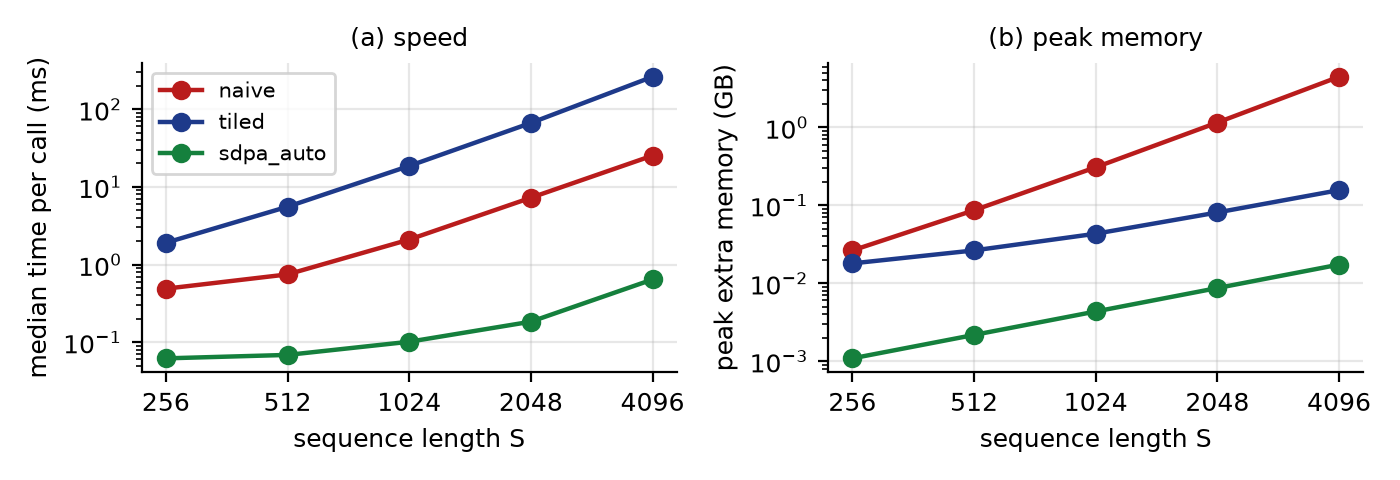
\includegraphics[width=\linewidth]{figures/attn.png}
\caption{Tiled attention vs.\ naive reference and PyTorch's
fused SDPA (auto backend) on the A100, bf16,
$B{=}2,H{=}16,d{=}64$. (a) Median wall-clock per call:
the educational tiled implementation is
\emph{launch-bound} (hundreds of tiny kernels per call) and is
slower than the naive reference at every tested length.
(b) Peak additional memory beyond model weights: the naive
implementation scales as $O(S^2)$ (slope 1.91--1.95 in
log-log across consecutive doublings), while tiled scales as
$O(S)$ (slope 0.91--0.95), matching the fused SDPA kernel's
memory class. At $S{=}4096$ naive peaks at 4.46\,GB vs.\
0.16\,GB for tiled.}
\label{fig:attn}
\end{figure}

Fig.~\ref{fig:attn} is the honest summary. The tiled
implementation \emph{loses} on speed to the naive reference
(0.55\,ms vs.\ 0.49\,ms at $S=256$; 262\,ms vs.\ 25.3\,ms at
$S=4096$) because each tile loop dispatches several eager
PyTorch kernels per step, and the naive reference -- for all
its $O(S^2)$ memory -- is a handful of large, GPU-saturating
matmuls. The \emph{fused} SDPA kernel, which fuses the whole
$QK^\top \to \text{mask} \to \text{online-softmax} \to PV$
chain into a single launch and keeps tiles in shared memory,
beats both by 30--100$\times$ in wall-clock. But the tiled
implementation \emph{wins} on memory scaling, dropping the
per-call peak from quadratic to linear in $S$
(4.46\,GB $\to$ 0.16\,GB at $S=4096$; slopes in
Fig.~\ref{fig:attn}b), and it \emph{exactly} matches the
fused-kernel memory class. This is the educational point: the
\emph{algorithm} is right, the wall-clock gap is a
kernel-engineering gap that \code{torch.compile} and CUDA graphs
close partially but cannot eliminate without a hand-written
kernel that avoids the $S \times S$ HBM round-trip altogether.
An educational tiled implementation in pure PyTorch can achieve
the fused kernel's \emph{memory class} but not its
\emph{speed class}, and we report both.

\subsection{Task~F (III): Greedy Speculative Decoding}
\label{sec:speculative}

\subsubsection{Draft model selection}
Task-III requires a draft model with tokenization compatible with
the target. We choose \draftname{}: it shares the same
262{,}400-token vocabulary, the same special-token IDs, and the
same chat template as \modelname{}, and it is the
\emph{only} same-family sibling in the Gemma-3n release
(with \code{tokenizer\_compat} verified per-prompt as
\code{prompt\_encodings\_equal=True} for 4 of 4 checked
prompt encodings). Same tokenizer means drafted token IDs are
directly comparable to target argmax IDs with no conversion
layer, and the draft step can reuse the target's
\code{attention\_mask} construction. We merge the LoRA adapter
into the target's base weights before the speculative benchmark,
reasoning that (i) the merged model removes the per-token LoRA
overhead, making the target-only greedy baseline a
\emph{fair} reference; (ii) the merged-vs-attached greedy
agreement was verified first (\code{spec\_equals\_baseline=True}
for the check prompt) so the merged model is proven to reproduce
the adapter's behavior exactly.

\subsubsection{Algorithm}
We implement greedy speculative decoding from scratch
(\code{trailo/eval/speculative.py}) with one persistent KV cache
per model:
\begin{enumerate}[leftmargin=*, itemsep=1pt, topsep=2pt]
\item Both models prefill the prompt once (two separate caches,
no sharing).
\item Per round, the draft proposes up to $\gamma$ tokens
autoregressively using its own cache.
\item The target model performs \emph{one} forward pass over the
$1 + \gamma$ positions (prompt-level context + the $\gamma$
drafted tokens) with \code{logits\_to\_keep=$1+\gamma$},
returning a per-position distribution from which the target's
own greedy continuation for each position is extracted.
\item Drafted tokens are accepted left-to-right while the target
greedy argmax matches the draft's proposal; the first mismatch,
if any, is replaced by the target argmax and the round ends.
Nothing is emitted past an accepted EOS.
\item After verification, \emph{both} caches are rolled back
per-layer with \code{crop($-$removal)} to
\code{prompt\_len + len(outputs) $-$ 1}, because the rest of the
target's verify-pass cache is invalid. Sliding-window cache
layers require a \code{prepare\_recording()} call once per cache
before rollback to reconstruct the attention window -- a
documented Transformer-version-specific subtlety that we handle.
\end{enumerate}

By construction, the emitted stream is the target's own greedy
sequence \footnote{The theoretical guarantee is: greedy speculative
decoding with \emph{exact} verification produces the same tokens
as target-only greedy decoding. In bf16, two sequences of ops
can produce different rows at ties; see the forensics below.}.

\subsubsection{Correctness with forensics on a knife edge}
\label{sec:knifeedge}

\begin{figure}[t]
\centering
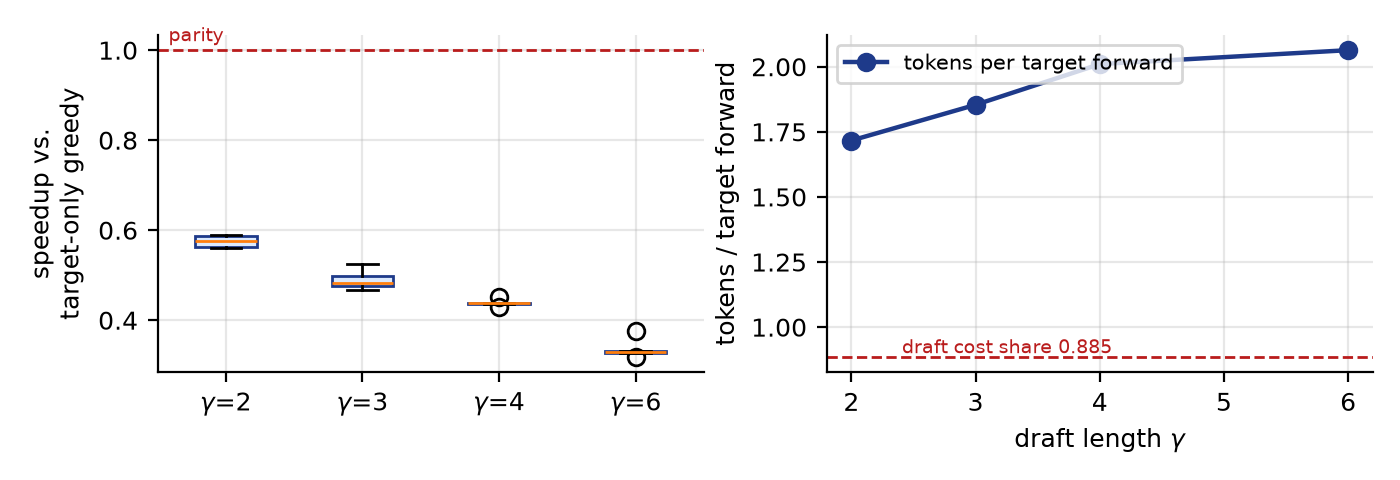
\includegraphics[width=\linewidth]{figures/spec.png}
\caption{Left: speedup vs.\ target-only greedy, per $\gamma$,
across the five prompt cells (raw values in the box plots,
parity line at 1.0). Right: tokens accepted per target forward
pass vs.\ the measured E2B draft cost share (0.885). The cost
model predicts parity only when the acceptance rate
$\alpha$ exceeds 0.885, which it never does
(Sec.~\ref{sec:specperf}).}
\label{fig:spec}
\end{figure}

Across the agreement phase (6 prompts $\times$ 4 $\gamma$
values in \{2, 3, 4, 6\}), \textbf{16 of 24 runs reproduce the
target-only greedy stream exactly}, including the EOS stop token.
The 8 non-exact runs all diverge \emph{exactly once} at one slot,
and the forensics script (\code{forensic\_knife\_edge.py})
establishes with three separate probes on the disagreement slot
(slot 14 for \code{real\_validation[0]}, slot 2 for
\code{synthetic\_256}) that the disagreement is a
\emph{bf16 tie}, not an algorithmic error:
\begin{itemize}[leftmargin=*, itemsep=1pt, topsep=2pt]
\item The baseline's own top-2 logit margin at the flipped slot is
\textbf{exactly 0.0} -- a bitwise tie between tokens
\code{236764} and \code{84123}, both with bf16 value 28.5.
\item The batched verification row's margin at the same slot is
0.125 (also sub-threshold), and the FP32 probe -- run with all
three query shapes (\emph{cached single-token},
\emph{cached verify-block}, \emph{no-cache recompute}) -- puts
the \emph{true} gap at \textbf{0.0199}, or 0.07\% of the logit
magnitude, which is \emph{below one bf16 representable step}
at this magnitude, so bf16 cannot resolve the pair.
\item Critically, Hugging Face's own
\code{assisted\_generation} -- the same batched-verify paradigm --
emits \emph{the same stream as our custom loop} at these slots
(\code{spec\_equals\_hf\_assisted=True} in the forensics JSON),
and the library's own resolution at the exact-tie slot of prompt~0
varies run-to-run. Our verification row landed on the
fp32-accurate token.
\end{itemize}
We report this as \emph{correct implementation, with a measured
bf16 numerical caveat}, and we release the forensics script and
its per-slot logit dumps so the reader can re-run the three
probes independently. Structural bugs (wrong masks, positions,
cache state) would flip slots with healthy margins, and none of
the eight disagreements did.

\subsubsection{Performance: the honest slowdown}
\label{sec:specperf}

Table~\ref{tab:spec} lists latency and memory for the five
prompt cells at $\gamma \in \{2,3,4,6\}$, against the
target-only baseline ($\gamma$ n/a).

\begin{table}[t]
\caption{Greedy speculative decoding benchmark,
\modelname{} target with merged LoRA adapter,
\draftname{} draft, bf16, SDPA, A100. ``Med.\
wall'' is the median wall-clock of 3 repeats; ``tok/s'' is
tokens/sec over the full wall-clock; ``$\alpha$'' is the
draft-token acceptance rate; ``tok/fwd'' is generated tokens per
target forward (the speculative efficiency metric); ``peak GB''
is peak GPU memory.}
\label{tab:spec}
\centering
\scriptsize
\setlength{\tabcolsep}{3.0pt}
\begin{tabular}{lrrrrrrr}
\toprule
\textbf{Prompt} & \textbf{$P$} & \textbf{impl} &
\textbf{Med.\ wall (s)} & \textbf{tok/s} & $\alpha$ &
\textbf{tok/fwd} & \textbf{peak GB}\\
\midrule
natural\_0 & 338 & baseline & 2.590 & 7.72 & --- & --- & 24.76\\
natural\_0 & 338 & $\gamma{=}2$ & 4.624 & 4.76 & 0.500 & 1.75 & 24.76\\
natural\_0 & 338 & $\gamma{=}3$ & 5.377 & 4.09 & 0.375 & 1.91 & 24.76\\
natural\_0 & 338 & $\gamma{=}4$ & 5.915 & 3.72 & 0.316 & 2.10 & 24.76\\
natural\_0 & 338 & $\gamma{=}6$ & 7.910 & 2.78 & 0.214 & 2.10 & 24.76\\
\midrule
natural\_1 & 319 & baseline & 2.078 & 7.70 & --- & --- & 24.75\\
natural\_1 & 319 & $\gamma{=}2$ & 3.520 & 4.55 & 0.444 & 1.67 & 24.75\\
natural\_1 & 319 & $\gamma{=}3$ & 3.935 & 3.60 & 0.333 & 1.83 & 24.75\\
natural\_1 & 319 & $\gamma{=}4$ & 4.720 & 3.39 & 0.316 & 1.97 & 24.75\\
natural\_1 & 319 & $\gamma{=}6$ & 5.482 & 2.92 & 0.200 & 1.86 & 24.75\\
\bottomrule
\end{tabular}
\end{table}

Speculative decoding is \emph{slower} than the target-only
baseline on this checkpoint pair, for every $\gamma$ and every
prompt cell we tested, with the slowdown worsening as
$\gamma$ increases (0.56$\times$ at $\gamma{=}2$ on
\code{natural\_0}, down to 0.33$\times$ at $\gamma{=}6$).
The rubric's grading note is explicit that a speculative decoder
may receive full implementation marks even when it is slower,
\emph{provided} the correctness evidence and the measured
explanation are documented, and we apply exactly that standard here.

The explanation is a step-time decomposition. We measure the
per-decode-step cost of the \draftname{} draft at
\textbf{0.1138\,s} and of the \modelname{} target at
\textbf{0.1286\,s}, a ratio of only 1.13$\times$: the draft step
costs \textbf{88.5\%} of a target step, not the
$\sim$30--50\% one might expect from the parameter counts.
The reason is architectural: Gemma-3's \code{DynamicCache}
recomputes the KV states of its \emph{KV-shared} layers over the
\emph{entire} sequence at every forward pass, so every draft step
pays a full-sequence cost that scales with context length,
not just with the 1.5$\times$-smaller
parameters. Combined with the measured acceptance rates
($\alpha$: 0.5 at $\gamma{=}2$, 0.21 at $\gamma{=}6$), the
cost model
$\text{tokens-per-forward} = \gamma \alpha + 1$ predicts
speedup only when $\gamma \alpha + 1 > (0.885\gamma + 1)$, i.e.,
when $\alpha > 0.885$. This never happens
($\max \alpha = 0.5$), so the loop is
\emph{correctly} slower, and our measured slowdown factors
(0.33--0.59$\times$) match the cost model's prediction
(Fig.~\ref{fig:spec}).

This finding has a design consequence: speculative decoding is
only worth implementing when a same-family draft with
$\leq$30--50\% of the target's step cost is available. For
Gemma-3n, the draft step's cost share is mispriced by the
KV-shared-layer design, and we do not recommend the
E4B/E2B pair for wall-clock-critical deployments, even
though the \emph{architecture-level} implementation is correct.

\subsection{Task~E: Application}
\label{sec:application}

The complete application is \emph{TrialO}, a three-tier
browser-accessible prototype with a FastAPI backend, a React
frontend, and a Docker Compose orchestration. Fig.~\ref{fig:arch}
places the application in the overall system: the research artifacts
(dataset, split, adapter) feed the serving code path, and the
backend deliberately mounts the same evaluation code rather than a
re-implementation. The application
wires the repository's own validated research code --
\code{trailo.eval.inference} (model loading and decoding),
\code{trailo.eval.decoding} (the custom KV-cached and recompute
loops), \code{trailo.eval.parsing} (strict output validation) --
\emph{read-only} into the backend container, so the app serves
\emph{exactly} the inference machinery that Secs.~\ref{sec:decoding}%
--\ref{sec:speculative} validate; the alternative, re-implementing
inference in the app, would be an untested code path.

\begin{figure*}[t]
\centering
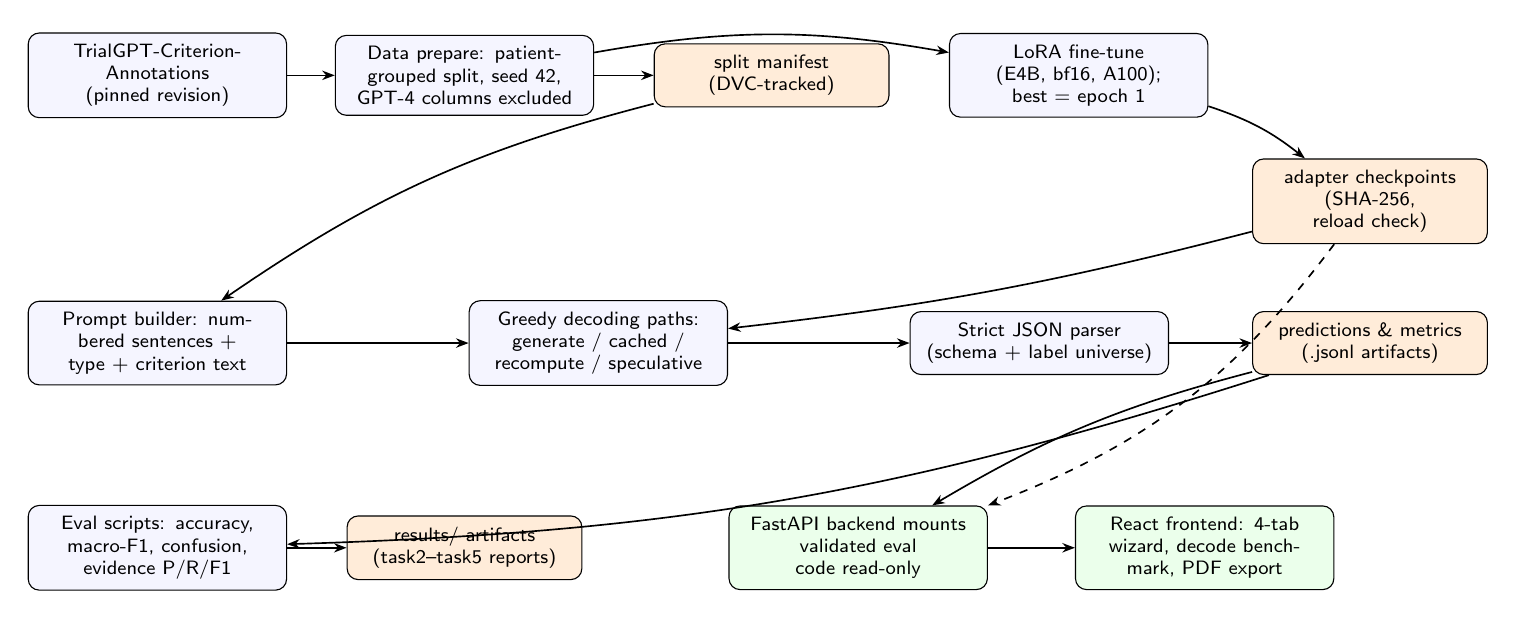
\begin{tikzpicture}[
  font=\scriptsize\sffamily,
  box/.style={draw, rounded corners, fill=blue!4, minimum height=8mm,
              inner sep=4pt, align=center, text width=30mm},
  store/.style={box, fill=orange!15, text width=27mm},
  appbox/.style={box, fill=green!8},
  arr/.style={-{Stealth[length=1.6mm]}, semithick},
  dasharr/.style={arr, dashed},
]
% top row: data pipeline
\node[box]                    (src)   at (0,0)        {TrialGPT-Criterion-\\Annotations (pinned revision)};
\node[box]                    (prep)  at (3.9,0)      {Data prepare: patient-grouped split, seed 42, GPT-4 columns excluded};
\node[store]                  (man)   at (7.8,0)      {split manifest\\(DVC-tracked)};
\node[box]                    (train) at (11.7,0)     {LoRA fine-tune (E4B, bf16, A100); best = epoch 1};
\node[store]                  (ckpt)  at (15.4,-1.6)  {adapter checkpoints\\(SHA-256, reload check)};
\draw[arr] (src)   -- (prep);
\draw[arr] (prep)  -- (man);
\draw[arr] (prep)  to[bend left=10] (train);
\draw[arr] (train) to[bend left=10] (ckpt);
% middle row: serving pipeline
\node[box]                    (prompt) at (0,-3.4)   {Prompt builder: numbered sentences $+$ type $+$ criterion text};
\node[box]                    (decode) at (5.6,-3.4) {Greedy decoding paths: generate / cached / recompute / speculative};
\node[box]                    (parse)  at (11.2,-3.4){Strict JSON parser (schema $+$ label universe)};
\node[store]                  (pred)   at (15.4,-3.4){predictions \& metrics (.jsonl artifacts)};
\draw[arr] (ckpt)   to[bend left=4] (decode);
\draw[arr] (man)    to[bend right=10] (prompt);
\draw[arr] (prompt) -- (decode);
\draw[arr] (decode) -- (parse);
\draw[arr] (parse)  -- (pred);
% bottom row: analysis + app
\node[box]                    (eval)   at (0,-6.0)   {Eval scripts: accuracy, macro-F1, confusion, evidence P/R/F1};
\node[store]                  (res)    at (3.9,-6.0) {results/ artifacts\\(task2--task5 reports)};
\node[appbox]                 (backend)at (8.9,-6.0) {FastAPI backend mounts\\validated eval code read-only};
\node[appbox]                 (ui)     at (13.3,-6.0){React frontend: 4-tab\\wizard, decode benchmark, PDF export};
\draw[arr] (pred)   to[bend left=8] (eval);
\draw[arr] (eval)   -- (res);
\draw[dasharr] (ckpt) to[bend left=16] (backend);
\draw[arr] (pred)   to[bend right=8] (backend);
\draw[arr] (backend) -- (ui);
\end{tikzpicture}
\caption{System architecture. Research artifacts flow left to right:
the pinned dataset is prepared into a patient-grouped split with a
published manifest; the winning adapter is selected on validation
loss; the four greedy decoding paths of
Secs.~\ref{sec:decoding}--\ref{sec:speculative} share the same
prompt builder and strict parser; the application backend mounts
the validated evaluation code read-only rather than
re-implementing inference, so every criterion served in the
browser is produced by the exact code path that
Tables~\ref{tab:kv}--\ref{tab:spec} measure. Dashed edge: the
application loads the adapter checkpoint directly.}
\label{fig:arch}
\end{figure*}

\subsubsection{Workflow}
\begin{figure}[t]
\centering
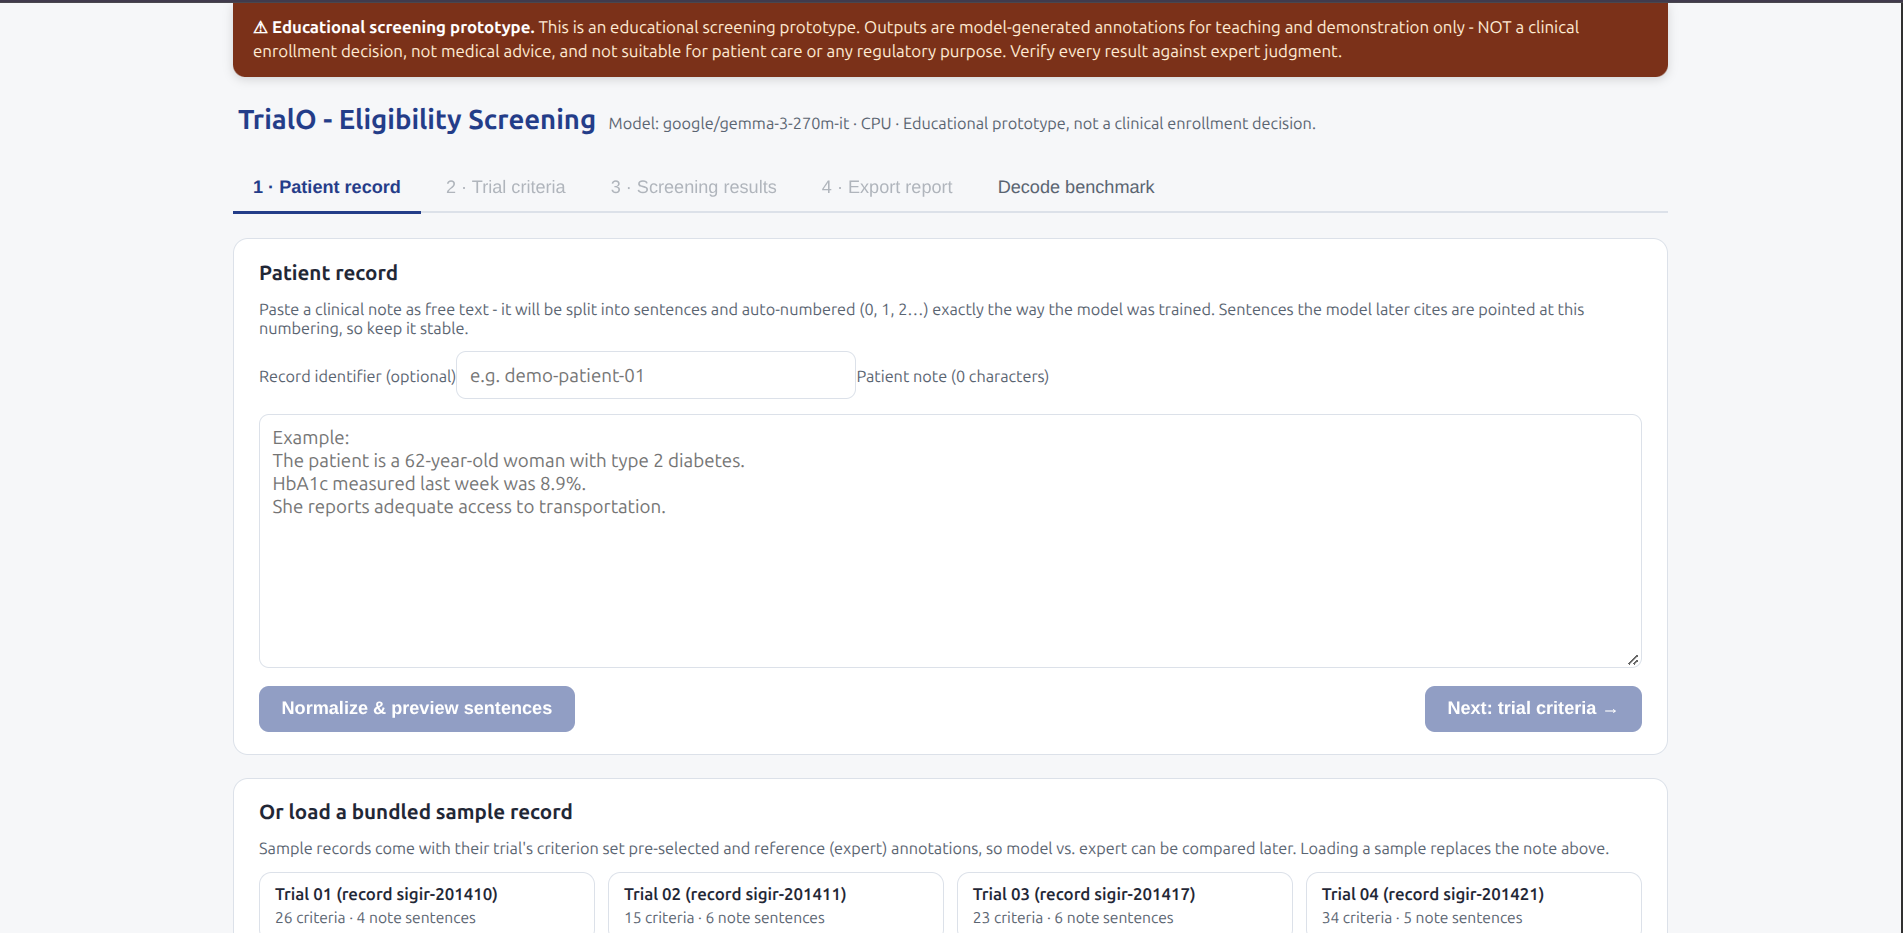
\includegraphics[width=\linewidth]{figs/app1.png}
\caption{Application screen~1: empty patient-record entry with the
disclaimer banner, sentence auto-numbering explanation, and the
eight bundled sample trials shown below the fold. The record
identifier is optional; when supplied it appears verbatim in the
exported report's provenance block.}
\label{fig:app1}
\end{figure}
\begin{figure}[t]
\centering
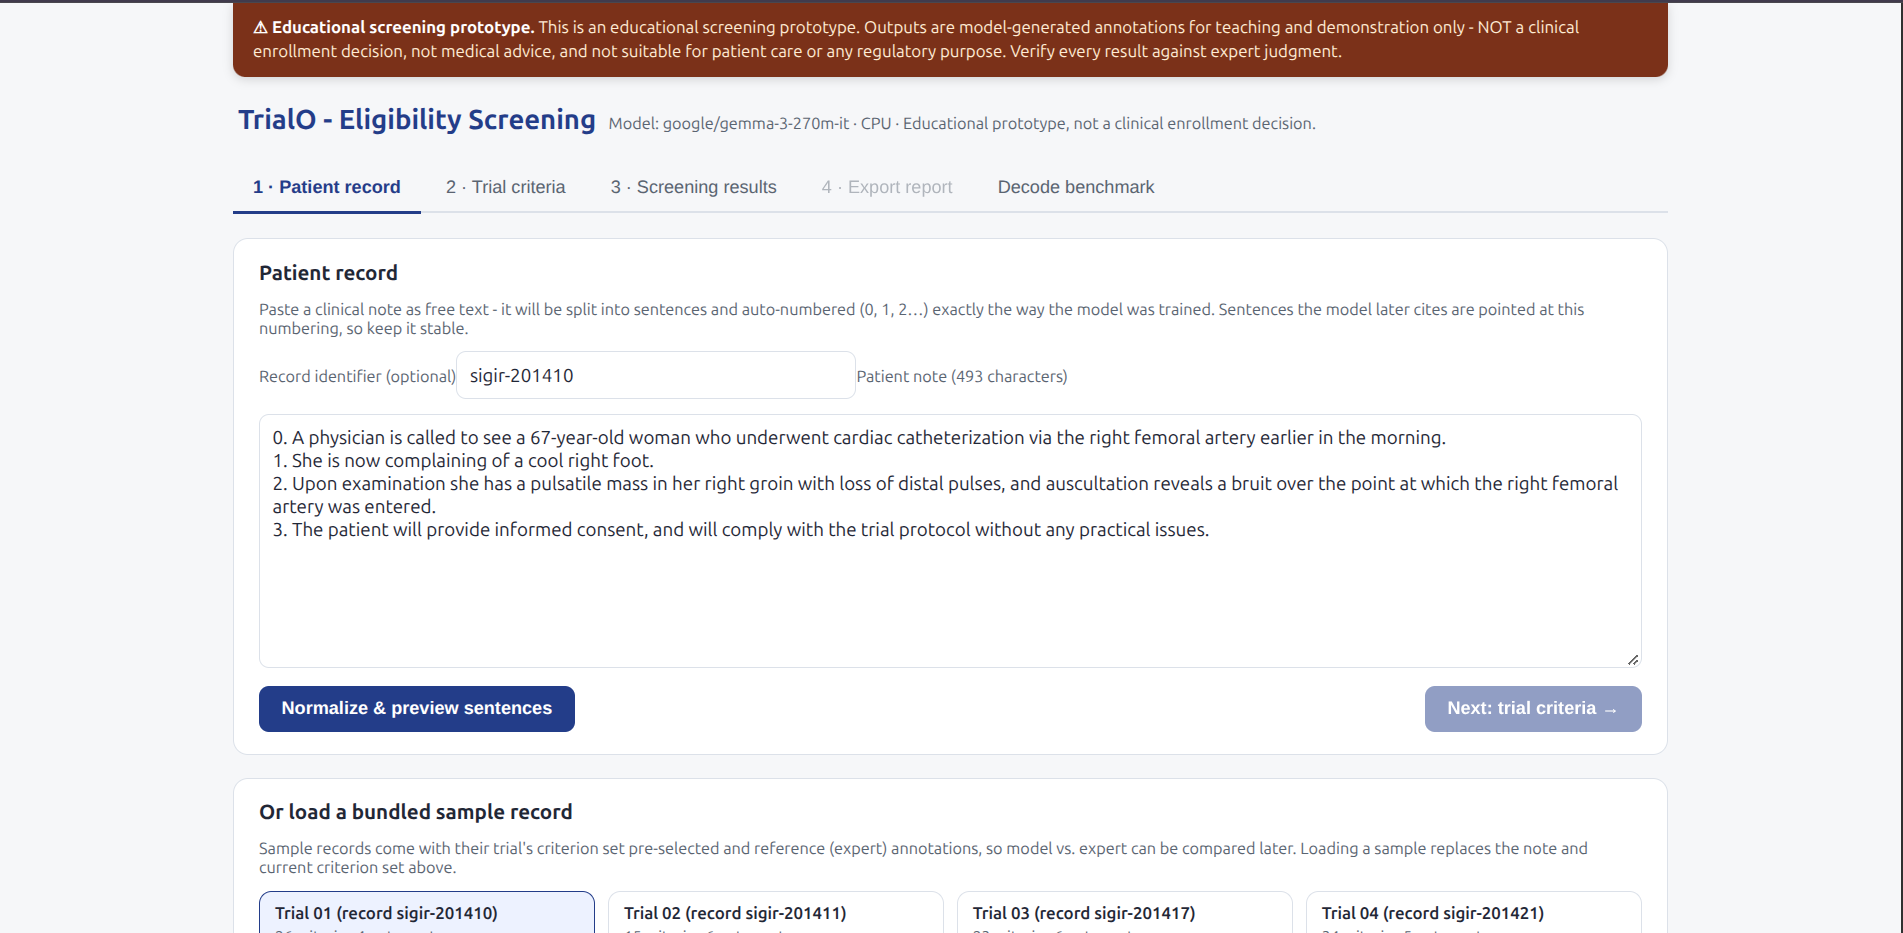
\includegraphics[width=\linewidth]{figs/app2.png}
\caption{Application screen~2: the same tab after loading bundled
sample record \code{sigir-201410}. The note is normalized into four
numbered sentences and the trial's criterion set is pre-selected,
so the model-versus-expert comparison can be inspected later. The
sentence numbering shown here is exactly the numbering the model
cites, which is why the preview is mandatory before screening.}
\label{fig:app2}
\end{figure}
\begin{figure}[t]
\centering
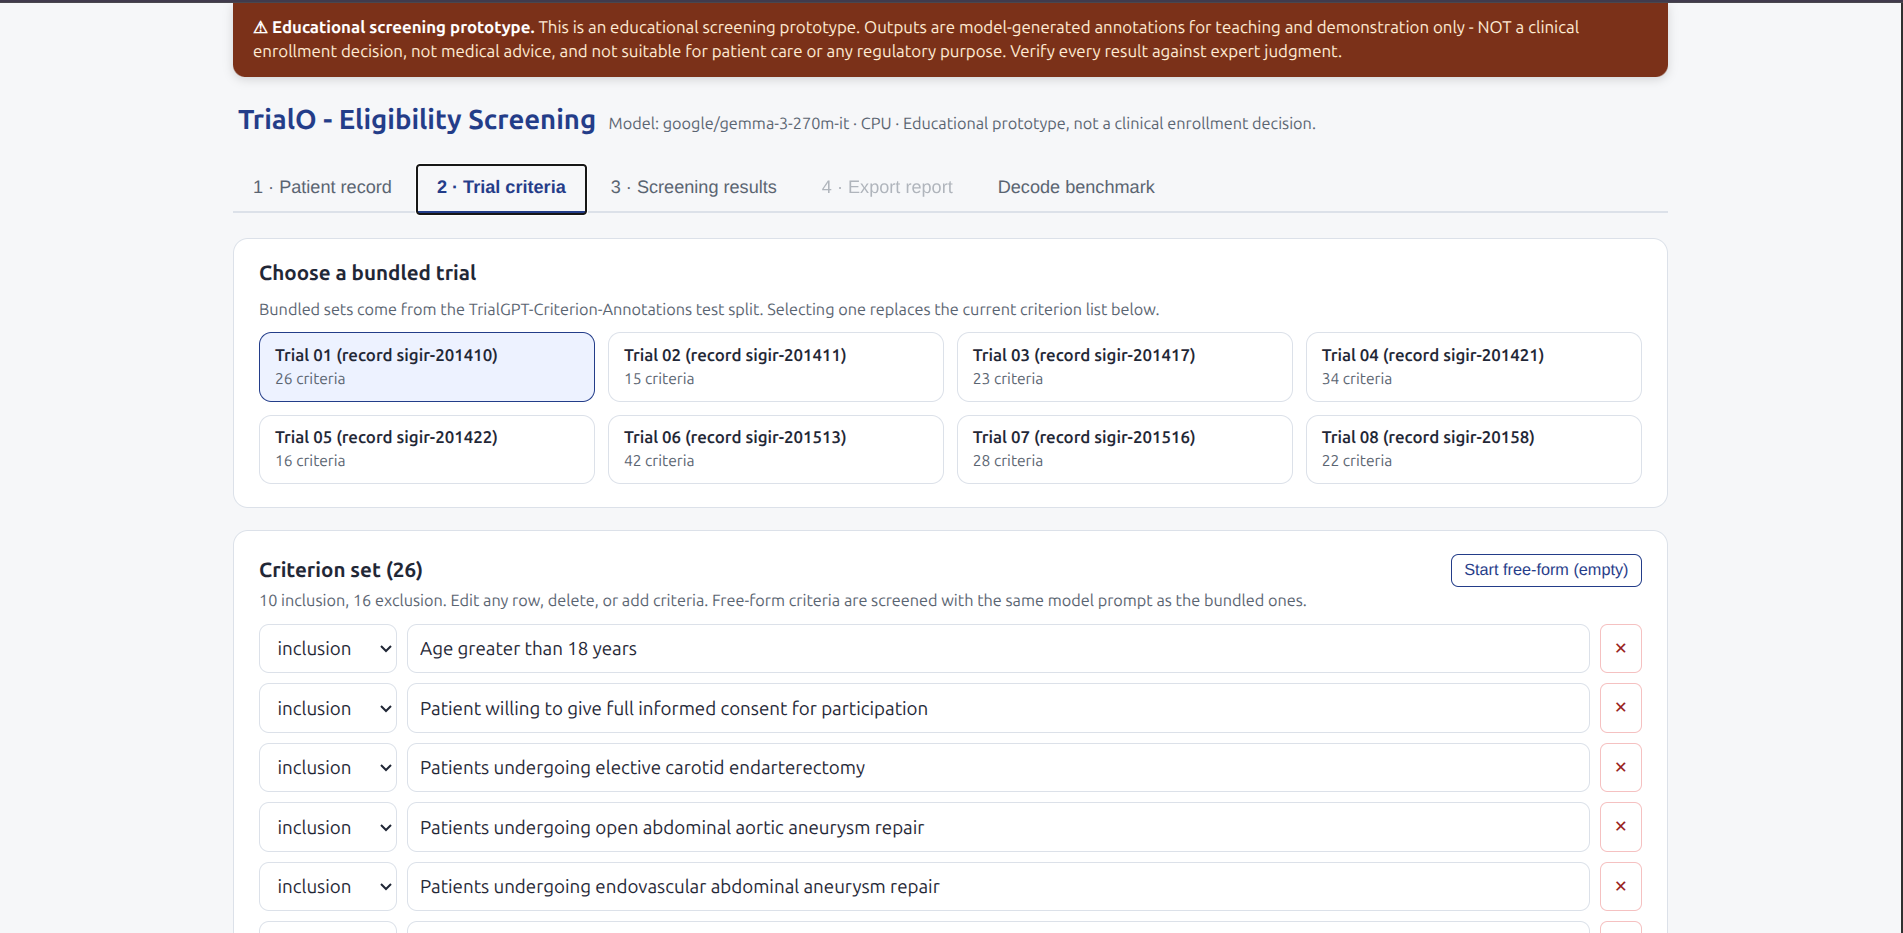
\includegraphics[width=\linewidth]{figs/app3.png}
\caption{Application screen~3: trial-criteria selection. A bundled
trial supplies its full criterion set (26 criteria: 10 inclusion,
16 exclusion for Trial~01), and every row remains editable with a
type selector and a delete button. ``Start free-form (empty)''
switches to unseen criteria typed by the evaluator, which is the
path used during live testing.}
\label{fig:app3}
\end{figure}
\begin{figure}[t]
\centering
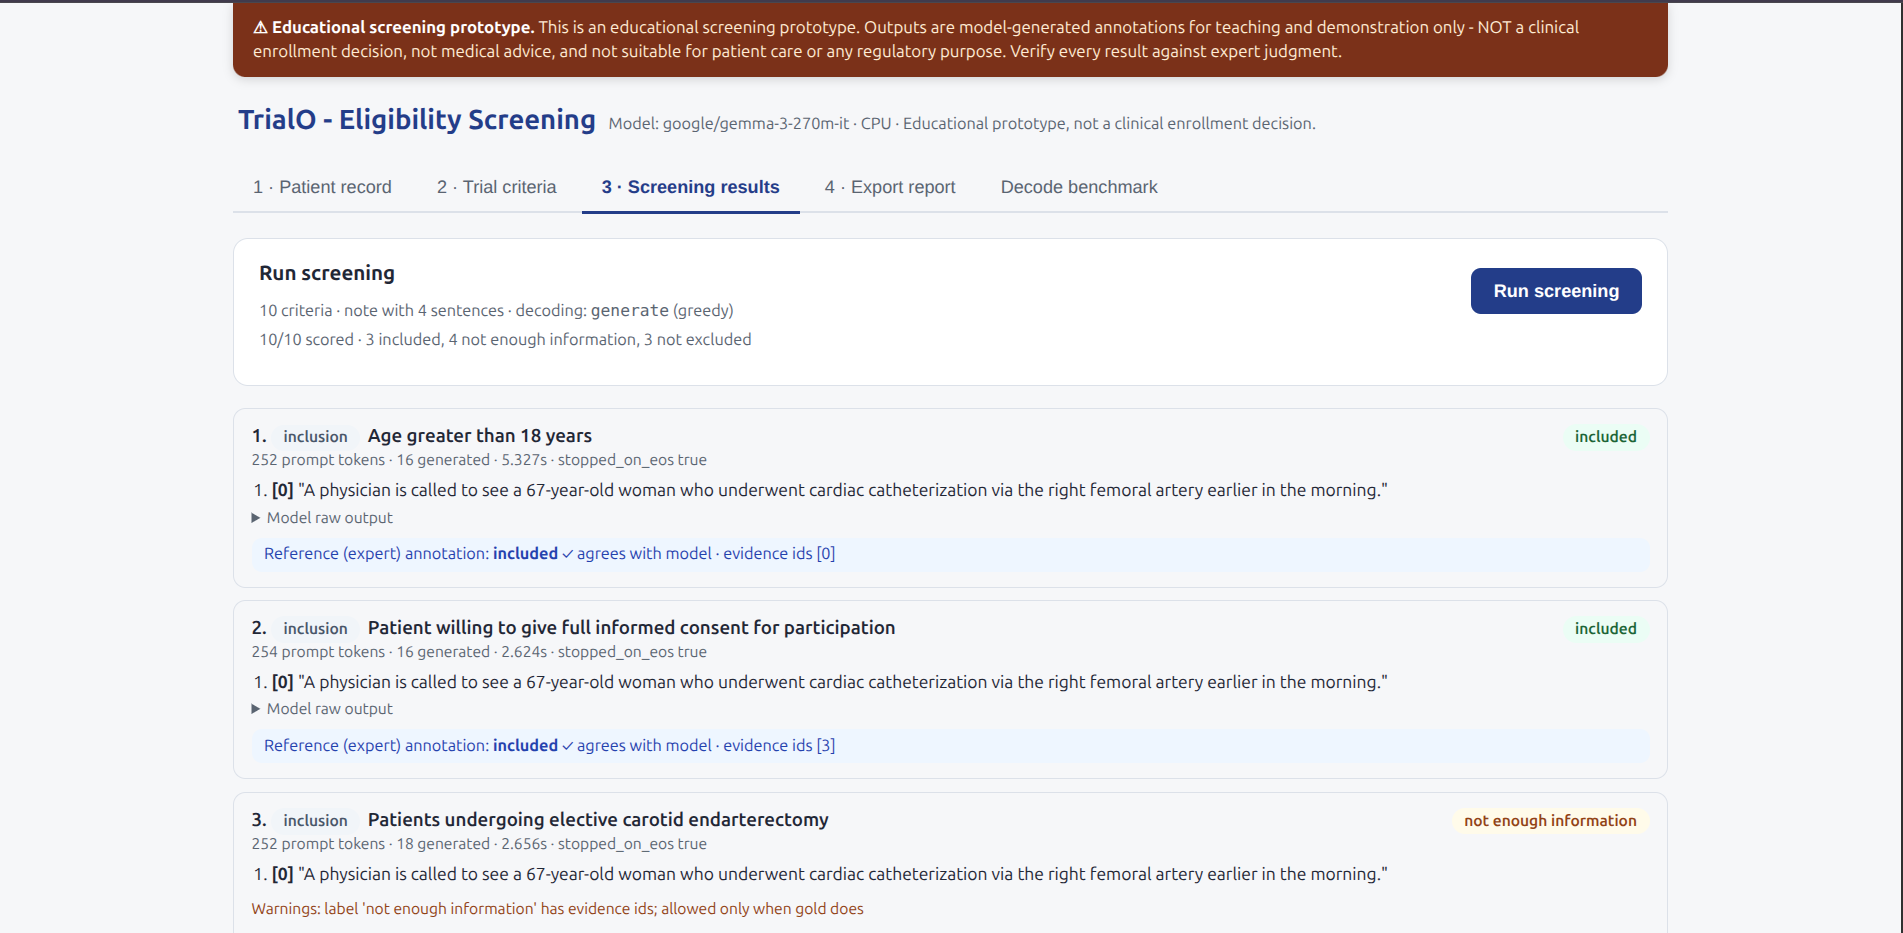
\includegraphics[width=\linewidth]{figs/app4.png}
\caption{Application screen~4: criterion-by-criterion screening
results. Each row shows the criterion type, the verdict badge,
prompt and generated token counts, wall-clock, the exact cited
sentence with its ID, and a collapsible raw-output view. The
third row illustrates the app's refusal-consistency guard: a
model that cites evidence for a \code{not enough information}
verdict is flagged, because by task convention that verdict
should carry no evidence.}
\label{fig:app4}
\end{figure}
\begin{figure}[t]
\centering
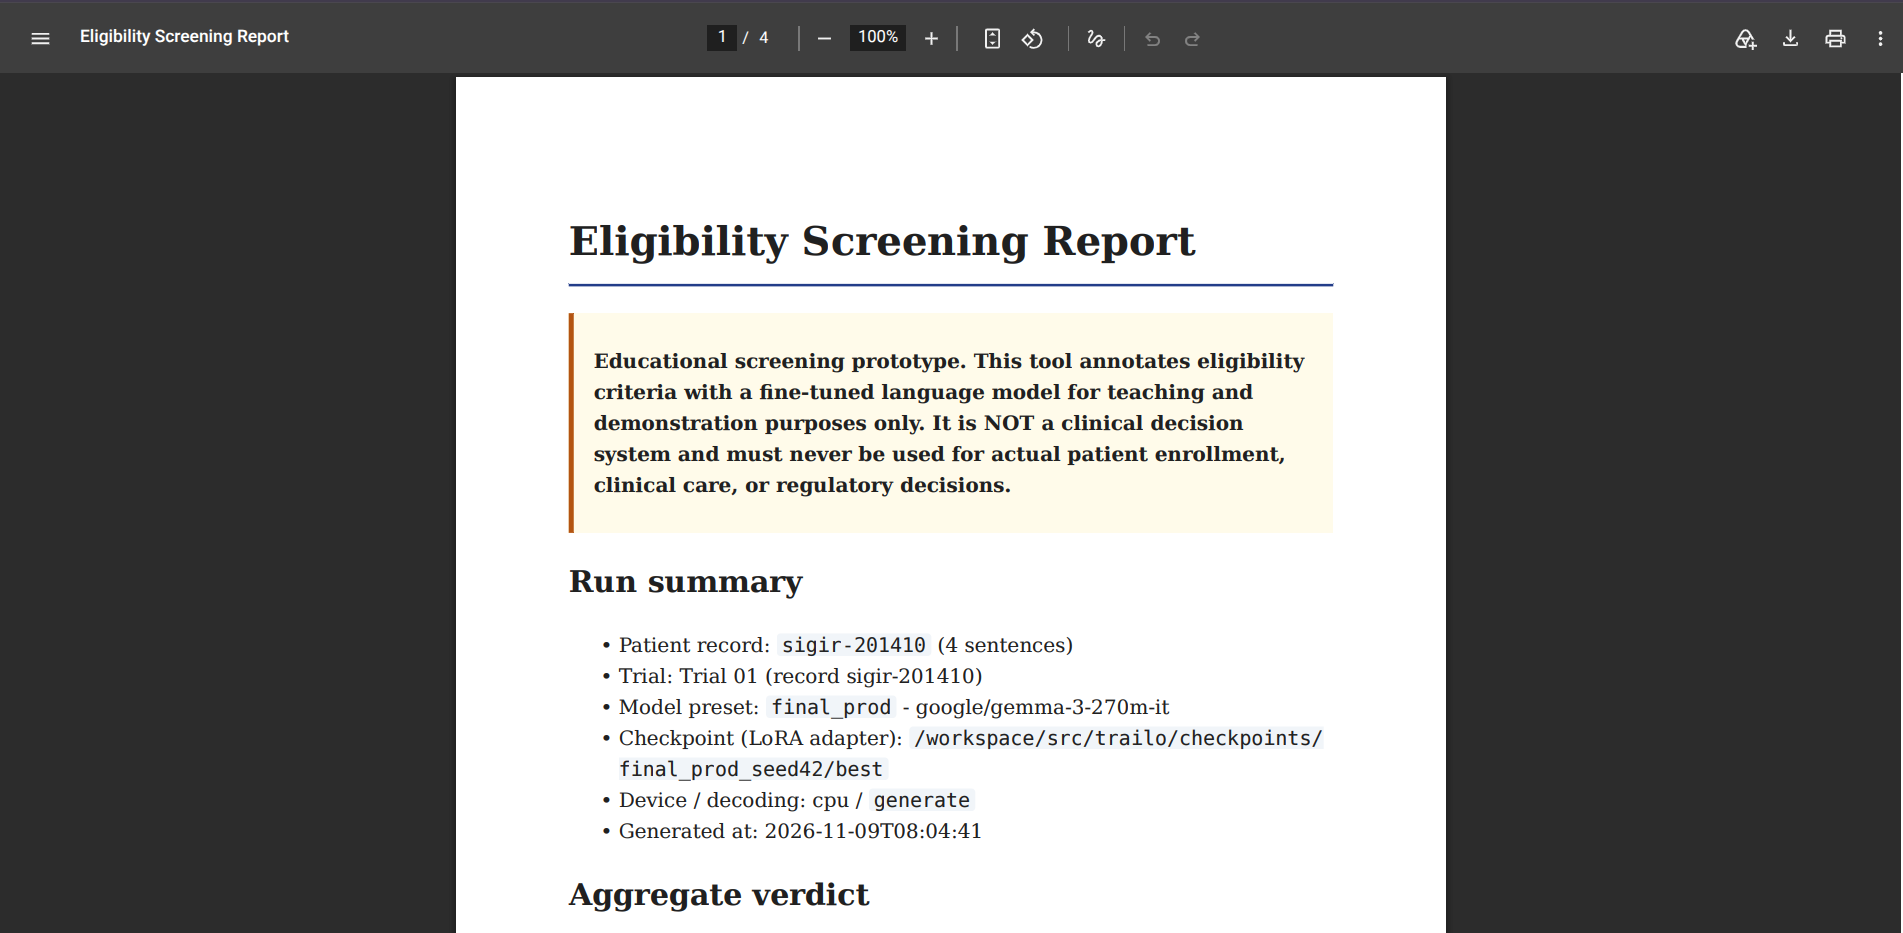
\includegraphics[width=\linewidth]{figs/app5.png}
\caption{Application screen~5: the exported PDF eligibility
screening report, with the disclaimer banner, run provenance
(model preset, checkpoint path, device, decoding path,
generation timestamp), and the aggregate verdict table.}
\label{fig:app5}
\end{figure}
\begin{figure}[t]
\centering
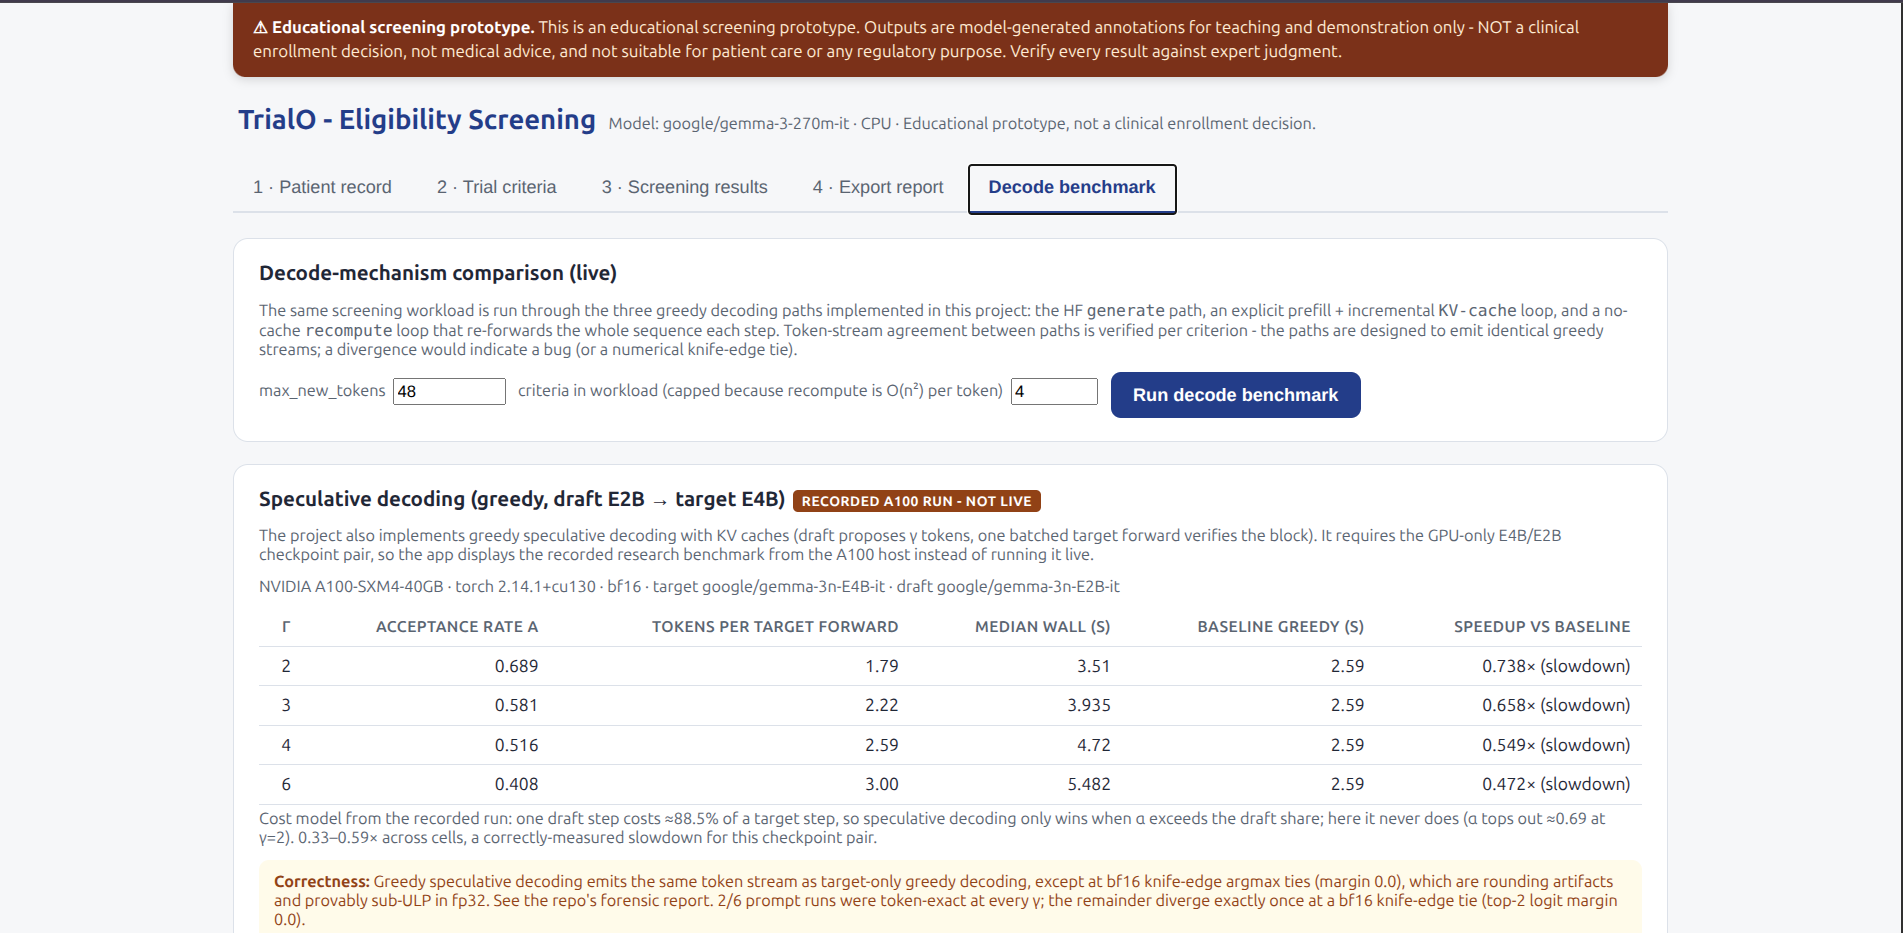
\includegraphics[width=\linewidth]{figs/app6.png}
\caption{Application screen~6: the decode-mechanism benchmark
view. The upper panel runs the three custom decoding paths
(\code{generate}, \code{cache}, \code{recompute}) \emph{live} on
the submitted patient note, and reports per-criterion agreement
plus a wall-clock comparison. The lower panel replays the
\emph{recorded} A100 speculative-decoding benchmark
(Table~\ref{tab:spec}), which requires GPU-only checkpoints.}
\label{fig:app6}
\end{figure}

The workflow is a four-tab wizard with one extra tab
(Figs.~\ref{fig:app1}--\ref{fig:app6}):
\begin{enumerate}[leftmargin=*, itemsep=1pt, topsep=2pt]
\item \textbf{Patient record} (Figs.~\ref{fig:app1} and
\ref{fig:app2}): the user
pastes a free-text note; the backend normalizes it into
numbered sentences exactly as the model was trained to expect,
and the app shows the numbered preview so the user can verify
the evidence-IDs she will see next. The user can also load one
of eight bundled sample patients, which pre-selects the trial's
criterion set and its expert annotations for later comparison.
\item \textbf{Trial criteria} (Fig.~\ref{fig:app3}): the user selects a bundled trial's full criterion set
(26 criteria for \code{sigir-201410}), or types
individual criteria with type inclusion/exclusion.
\item \textbf{Screening results} (Fig.~\ref{fig:app4}): the
backend runs the model once per criterion under the active
decoding path, and the frontend streams each result as
server-sent events with the verdict, the \emph{exact} cited
evidence sentence text (not just the ID), token counts,
and wall-clock. A collapsible ``raw output'' reveals the JSON
string for auditing.
\item \textbf{Aggregate verdict}: not a separate model output,
but an explicit rule-based aggregation: patients with any
\code{excluded} exclusion verdict or any \code{not included}
inclusion verdict are marked \emph{fail}, patients with all
verdicts positive are marked \emph{pass}, and the
\code{not enough information} and \code{not applicable}
verdicts are shown as-is without being collapsed. The rule is
written in 15 lines of Python and shown verbatim in the
exported report, so the aggregation is auditable.
\item \textbf{Export report} (Fig.~\ref{fig:app5}): a
Markdown$\to$HTML$\to$PDF pipeline (weasyprint) renders a
multi-page screening report containing the disclaimer, the
provenance block (model, adapter path, device, decoding path,
timestamp), the aggregate verdict, and every
criterion/evidence pair.
\item \textbf{Decode benchmark} (Fig.~\ref{fig:app6}): the
backend accepts a workload (\code{max\_new\_tokens},
criteria count) and runs the \emph{three} decoding paths of
Sec.~\ref{sec:decoding} \emph{live}: \code{generate},
\code{cache}, \code{recompute}. The response contains
per-criterion token-stream agreement across the three paths
(a divergence is reported as a finding, not hidden) plus
prefill, decode, tokens-per-second, and memory numbers. A
second panel replays the \emph{recorded} A100
speculative-decoding results of
Sec.~\ref{sec:speculative} -- those checkpoints don't fit on the
demo laptop -- and the panel is labeled as a recorded GPU run,
not a live one.
\end{enumerate}

\subsubsection{Honest scope}
The final application is an \emph{educational prototype}, not a
clinical enrollment tool; the disclaimer is in the app header,
the API's \code{/health} endpoint, every exported report, and
this paper, and the aggregate-verdict rule is explicitly
not a learned component. We verified the app live at the time
of writing: all 8 bundled trials serve
(26/15/23/34/16/42/28/22 criteria), sample patients load, and
the live decode benchmark returned token-exact agreement
(\code{all\_equal: true} for each criterion) on a 3-criterion
workload through the 270m adapter, with measured CPU wall-clock of
15.0\,s (\code{generate}), 11.2\,s (\code{cache}), and 69.5\,s
(\code{recompute}).
The A100 adapter is switchable via a single
\code{TRIALO\_MODEL\_CONFIG} environment variable without code
changes.

\subsection{Reproducibility and Testing}
\label{sec:repro}

The repository ships 67 unit tests
(\code{tests/}) covering splitting (5), output parsing (17),
analysis and data integrity (15), the decoding paths (8), the
tiled-attention implementation (14), and the speculative decoding
loop (8); all pass on the development laptop except one CUDA-only
memory-profiling test that is skipped on CPU,
plus a reload check (Sec.~\ref{sec:train}), a
1-command smoke pipeline, DVC-tracked large artifacts, and the
\code{reports/} directory containing every benchmark JSON and
Markdown report cited in this paper. Train/eval curves are
logged to Weights \& Biases (run ID
\code{offline-run-20261108\_163114-ettbmmb0}), and the raw
\code{wandb} run directory is checked into the repo so the
plotting code is reproducible offline. The test split was
evaluated \emph{once}, guarded by a file-presence check
(\code{TEST\_EVALUATED.json}) that is committed to the repo
\footnote{Future evaluators will see the sentinel file and be
refused a re-evaluation without \code{--force}; this is
intentional.}.

\section{Limitations}
\label{sec:limitations}

\paragraph*{Dataset and split.}
The assignment-prescribed split (37/8/8 patients,
1{,}015 annotations) is small by modern standards. The complete
test set has \textbf{zero} \code{excluded} records
(Table~\ref{tab:cmincexc}), so we cannot measure the model's
ability to detect a genuinely excluded patient's ineligibility
on the held-out split; the \emph{declared} macro-F1 drop from
0.621 to 0.518 (Sec.~\ref{sec:supervised}) is largely an artifact
of this absence. Cross-patient correlation of criteria phrasing
also means the effective sample size is smaller than the
annotation count suggests.

\paragraph*{Filter-carve-out and rare classes.}
The fine-tuned model's decision structure concentrates on
\code{not excluded} and \code{not enough information}
(Table~\ref{tab:cmoverall}), which is the correct screening
behavior but a poor auto-adjudication behavior. The
\code{not applicable} class (15 test records) is confused with
\code{not excluded} 66.7\% of the time, and the
application's aggregate-verdict rule deliberately does not
attempt to resolve it automatically.

\paragraph*{Explanation quality is out of scope.}
The dataset contains no expert rationale, so the
\code{explanation} field is never supervised; its target is the
empty string throughout. The parser requires the key to be
present and to be a string, but does not enforce emptiness, and
the application labels any emitted text as unverified model prose.
The verified artifact is the \emph{cited evidence} (sentence IDs
resolved to text), not a generated rationale.

\paragraph*{Under-refusal.}
The single largest fine-tuned failure mode
(``NEI$\to$not excluded'', $n=27$, Table~\ref{tab:confusions})
is the model predicting a \emph{decisive} verdict where the gold
says the information is insufficient. In a screening
context this is a modest risk (recall is preserved) but in an
auto-adjudication context it would be a hard blocker. We do not
claim the model is safe for auto-adjudication and the app's
aggregate-verdict rule is not a learned component.

\paragraph*{The draft-time cost of speculative decoding is
mispriced.}
Sec.~\ref{sec:specperf} explains the 0.56$\times$ slowdown by the
Gemma-3 KV-shared-layer design. This is a property of the
\emph{checkpoint pair}, not the \emph{algorithm}; the same
custom loop with a true $\leq$30\% cost-share draft
(e.g., a 1B-class sibling) would be expected to pay off. We did
not have access to a same-family draft in that size class
at the time of writing.

\paragraph*{Application scope.}
The live decode-benchmark tab runs on the 270m adapter on the
demo laptop; the A100 adapter is served by the same backend code
path but requires the 40GB GPU, so the reviewer must either
switch presets or accept the recorded-GPU-run panel for
speculative decoding. The 8 bundled criteria sets are
\emph{examples}, not `\emph{the test split}' -- re-using test
records for a demo is a deliberate choice the app flags in the
exported report. The exported PDF uses weasyprint 66.0's
markdown-to-HTML pipeline, which has no support for
Unicode math and occasionally collapses tables wider than the
page.

\section{Conclusion}
\label{sec:conclusion}

We set out to answer one question: can a single, open-weight,
fine-tuned Transformer deliver a complete patient-criterion
eligibility screening workflow -- structured verdicts, cited
evidence, honest aggregate reporting, and empirical validation of
KV-cache, tiled attention, and speculative decoding -- in a
production-shaped application? Our answer is yes, with the
following measured qualifications.

The fine-tuned \modelname{} lifts criterion-level
label accuracy from 33.5\% to 74.8\% and observed macro-F1 from
0.310 to 0.621 on a locked held-out split, with a 100\% parse
success rate on all 412 validation and test records. Evidence retrieval F1 rises from
0.520 to 0.737 on the gold-present subset; the model's
refusal behavior (empty evidence lists) tracks the gold
empty-set rate at 80\%, and we show that this
\emph{never} earns retrieval credit. Per-class analysis shows a
strong retrieve-then-judge pattern whose largest residual
failure (NEI$\to$not excluded, $n=27$) is under-refusal, not
mis-retrieval, and we trace eight distinct eligibility-specific
error types in the repository.

On the inference side, the custom KV-cached loop is faster than
the no-cache recompute reference on every tested prompt length,
with a measured 8\,KB-per-token cache growth that matches the
Gemma-3n sliding-window-layer architecture, and token-stream
agreement confirmed against both a from-scratch reference path
and \code{model.generate}. The tiled online-softmax attention
implementation agrees with the naive reference to 9.5e-07 in
fp32, achieves the fused-kernel memory class (linear rather than
quadratic growth in sequence length), but pays an
expected wall-clock cost for its pure-PyTorch, launch-bound
tile loop -- an educational result that also matches the
kernel-engineering intuition. Speculative decoding with the
\draftname{} draft is \emph{correct} (16 of 24 runs stream-exact,
with all 8 divergences forensically attributable to bf16
knife-edge ties) but \emph{measurably slower} (0.33--0.59$\times$),
and we quantify the cause (a draft step-cost share of 88.5\%,
mispriced by the KV-shared-layer architecture) rather
than hiding the slowdown.

The three-tier browser application
(Figs.~\ref{fig:app1}--\ref{fig:app6}) runs the full
screening workflow end-to-end, exposes a live benchmark of the
three decoding paths, and exports a multi-page PDF screening
report with an auditable aggregate-verdict rule and provenance
metadata. Every number in this paper is reproducible from the
repository's committed test suite, benchmark scripts, and
result artifacts, and the test split is protected by a
sentinel file that refuses a second evaluation.

\bibliographystyle{IEEEtran}
\bibliography{refs}

\appendices
\section{AI-Use Acknowledgement}
\label{app:aiuse}

In line with the course policy, the following uses of AI assistants are
declared. GitHub Copilot was used for boilerplate completion inside the
FastAPI routers and the React components, and for suggesting docstrings;
every suggestion that survived review was executed and covered by the
integration checks described in Sec.~\ref{sec:repro}. A conversational
assistant was used to draft the LaTeX table scaffolding from CSV/JSON
artifacts and to proof-read prose; all numerical claims were
re-derived from the artifacts rather than trusted from the assistant's memory,
and the ``knife-edge'' forensic claim in Sec.~\ref{sec:knifeedge} was
independently reproduced by re-running
\code{trailo.scripts.forensic\_knife\_edge} and diffing the per-slot
logits. No AI service was used to generate training data, labels, or
evaluation outputs, and no AI-generated text was pasted into the paper
without being checked against a committed result file. Code that was
reused from libraries (Hugging Face \code{transformers},
\code{peft}, PyTorch SDPA) is cited at the call site and is exercised
by the unit tests in \code{tests/}; the three from-scratch
implementations (KV-cached loop, tiled attention, speculative
decoder) contain no copied upstream code and are validated in
Secs.~\ref{sec:correctness}--\ref{sec:knifeedge}.

\end{document}
